\documentclass[11pt,a4paper]{article}
\usepackage[margin=2.3cm]{geometry}
\usepackage{amsmath,amssymb,graphicx,booktabs,hyperref,xcolor,caption,float}
\usepackage[T1]{fontenc}
\usepackage[round]{natbib}
\hypersetup{colorlinks=true,linkcolor=blue!50!black,urlcolor=blue!50!black,citecolor=blue!50!black}
\captionsetup{font=small,labelfont=bf}
\graphicspath{{../../plots/method_unified/}}
\newcommand{\vect}[1]{\boldsymbol{#1}}
\newcommand{\R}{\mathcal{R}}
\newcommand{\code}[1]{\texttt{#1}}

\title{Colour evidence for a same-redshift quasar companion:\\ the unified 41-band model (October 2026)}
\author{Internal method note, \code{qso\_pcolor}}
\date{4 October 2026}

\begin{document}
\maketitle

\begin{abstract}
A quasar has a spectroscopic redshift $z_0$, and a point source lies a few arcseconds away.
This note describes how \code{qso\_pcolor} measures, from broad-band photometry alone, how
strongly the companion's colours support the hypothesis that it is itself a quasar at $z_0$. The
method compares four populations: quasars at $z_0$, quasars at other redshifts, everything else
in the imaging catalogue (the background, mostly stars), and a broad catch-all. It accepts any
subset of 41 bands from seven surveys that includes Legacy Surveys $r$ at signal-to-noise $\geq10$.
One latent model, shared by the northern and southern Legacy Surveys, describes all bands, and
photometry is corrected for Galactic extinction. Two quasar models are provided: quasar colours
independent of apparent magnitude (the XDQSO design; the default), or free to depend on it. The
background is modelled as in XDQSO, by separate fits in eight bins of Legacy $r$, after removing
likely quasars from its training sample; its component weights vary smoothly with Galactic
position. On held-out stars this background describes the data better than the joint model it
replaces in every magnitude bin ($+4.9$\,nat per object at $r<17$, $+0.2$ at $r>23$). On held-out
quasars and background objects it ranks as well (AUC 0.976 and 0.980), finds more quasars, and
calls fewer background objects quasars. This note describes the candidate bundles of 3 October 2026;
it replaces the version of 2 October and the earlier \code{docs/method/method.tex}.
\end{abstract}

\tableofcontents
\newpage

%======================================================================
\section{Summary of what is delivered}
%======================================================================
\begin{itemize}
\item \textbf{Two candidate bundles} (3 October 2026, not yet promoted):
  \url{models/multisurvey_psf/work/stellar_binned/20261003/bundles/independent} (quasar colours
  independent of apparent magnitude; the intended default) and \code{.../dependent} (quasar colours
  free to depend on it). The promoted pointers \code{current} and \code{current\_magdep} still name the
  2 October bundles, which differ only in the background model, the faint limit and the support
  recalibration. Load with \code{UnifiedPSFModel.load(...)}.
\item \textbf{Inputs.} Any subset of 41 bands (SDSS $ugriz$; Legacy Surveys DR9 South and
  North $g,r,z,W1,W2$; AllWISE $W1$--$W4$; Pan-STARRS1 $grizy$; NSC $ugrizY{+}VR$; SkyMapper
  $uvgriz$; VHS $YJHK_s$) that contains Legacy $r$ at $S/N\geq10$, as catalogued fluxes or magnitudes
  with errors; candidate RA and Dec; the primary's redshift $z_0$; morphology and blend information.
  Fainter sources, and sources without Legacy $r$, are flagged and not scored (Section~\ref{sec:faint}).
\item \textbf{Output.} A ranking statistic $\log\R$ (Section~\ref{sec:question}), evidence and posterior
  quantities, a quasar-support percentile, and explicit eligibility and quality flags.
\item \textbf{Main results.} Section~\ref{sec:validation}. The binned background fits held-out stars far
  better than the joint background it replaces (Table~\ref{tab:bkgdensity}, Fig.~\ref{fig:stellarcc}).
  Against the promoted bundles on the same held-out objects, ranking is unchanged ($\Delta$AUC
  $-0.0006$ and $+0.0003$), recall at $p_{\rm quasar}>0.5$ rises by 2.3 and 1.9 points, and the fraction of
  background objects with $p_{\rm quasar}>0.5$ falls (Table~\ref{tab:compare}). On artificial colour
  grids the spurious high-quasar points of earlier models (up to 79) drop to 1 and 0. $p_{\rm quasar}$
  is consistent with the observed quasar fraction in the mid range and mildly overconfident above
  0.97 (Section~\ref{sec:calib}).
\end{itemize}

%======================================================================
\section{Notation and glossary}\label{sec:notation}
%======================================================================
\subsection{Symbols}
\begin{center}\small
\begin{tabular}{p{0.17\textwidth}p{0.75\textwidth}}
\toprule
Symbol & Meaning (units) \\
\midrule
$z_0$ & spectroscopic redshift of the primary quasar \\
$z$ & redshift of a hypothetical companion quasar \\
$\vect{y}$ & observed native luptitudes of a source in the bands it has (mag; Section~\ref{sec:photometry}) \\
$\vect{C}$ & measurement covariance of $\vect{y}$ (mag$^2$; diagonal in practice) \\
$\vect{x}$ & latent, noise-free luptitudes in the 36 shared coordinates (mag) \\
$H,\ \vect{b},\ T$ & observation operator: $\vect{y}=H\vect{x}+\vect{b}+\vect{\epsilon}$, with extra instrumental scatter $\vect{\epsilon}\sim N(0,T)$ \\
$m_{\rm ref}$ & luptitude of the reference band, Legacy $r$, on which colours are conditioned (mag) \\
$a$ & index of the reference band \\
$E$ & SFD98 reddening $E(B-V)$ at the source position (mag) \\
$R_j$ & extinction coefficient of band $j$, $A_j/E$ \\
$\ell,\ b$ & Galactic longitude and latitude (deg) \\
$\Sigma_Q(z,m)$ & quasar surface density per unit redshift and magnitude (deg$^{-2}$\,mag$^{-1}$) \\
$\Sigma_B(m)$ & background surface density per unit magnitude (deg$^{-2}$\,mag$^{-1}$) \\
$\eta$ & catch-all share of the background intensity (dimensionless) \\
$\lambda_X$ & intensity of hypothesis $X$: surface density times colour likelihood \\
$\R$ & ranking statistic, Eq.~(\ref{eq:R}) (per unit redshift) \\
$\Delta z_{\rm eff}$ & effective width of the declared redshift window, \code{dz\_match\_eff} \\
$K$ & number of Gaussian components in a mixture \\
$w,\ \nu$ & covariance-prior scale ($10^{-3}$\,mag$^2$) and strength ($1$) \\
\bottomrule
\end{tabular}
\end{center}

\subsection{Terms}
\begin{description}\small
\item[Luptitude.] The inverse hyperbolic sine magnitude of \citet{Lupton1999},
  \[m=22.5-\frac{2.5}{\ln 10}\left[\sinh^{-1}\!\left(\frac{f}{2s}\right)+\ln s\right],\]
  for flux $f$ in the band's native unit and softening $s$. It equals the ordinary magnitude for $f\gg s$ and stays finite for zero or negative flux.
\item[Native system.] A band's own catalogue calibration. No band is converted into another survey's system.
\item[Slice.] The quasar model for redshifts within $\pm0.1$ of a centre $z_k$, for $z_k=0.15,0.25,\dots,4.35$ (43 slices; neighbouring slices overlap).
\item[Reference band.] Legacy DR9 $r$: the southern band where observed, otherwise the northern one.
  Colour likelihoods are conditioned on it, and the background bins are defined in it. Every scored
  source has it at $S/N\geq10$ (Section~\ref{sec:faint}).
\item[Role.] Every training object belongs to one sky-based role: \emph{fit} and \emph{select} (training),
  \emph{calibration} (catch-all shares and support threshold), or \emph{test} (validation). Roles are fixed
  in advance and never reassigned.
\item[Background.] Every point source in the imaging catalogue that is not a quasar. It is dominated
  by stars and is fitted empirically. Its training sample excludes known quasars and likely quasars
  (Quaia members and WISE AGN colours; Section~\ref{sec:background}).
\item[Catch-all.] A broad Student-$t$ density with a small share of the background intensity. It
  explains objects that neither the quasar nor the background mixture fits, so that Gaussian tails do
  not decide their classification.
\item[Support percentile.] For a candidate and $z_0$, the fraction of simulated quasars at $z_0$, with
  the candidate's own errors, whose conditional density is lower than the candidate's. A small value
  means the colours are unusual for a quasar at $z_0$.
\item[Held-out density.] The mean, over test objects, of the conditional log density
  $\ln p(\vect{y}_{\rm other}\mid m_{\rm ref})$ (nat per object, density per mag$^{N-1}$). Higher is better.
\item[AUC.] The probability that a random test quasar ranks above a random test background object on
  $\log\R$. Objects the scorer declines to rank are placed at the bottom.
\end{description}

%======================================================================
\section{The question and the ranking statistic}\label{sec:question}
%======================================================================
Four hypotheses compete for a companion with photometry $\vect{y}$ near a primary at $z_0$
(Fig.~\ref{fig:schematic}):
\begin{enumerate}
\item $Q(z_0)$, a quasar at the primary's redshift, within a declared window;
\item $Q(z\neq z_0)$, a quasar at any other redshift;
\item $B$, a member of the background population;
\item $U$, the catch-all.
\end{enumerate}
Each hypothesis has an intensity, a surface density times a likelihood. With reference magnitude
$m$ and conditional colour likelihoods,
\begin{align}
\lambda_{Q}(z) &= \Sigma_Q(z,m)\,p(\vect{y}\mid Q,z,m), \\
\lambda_B &= (1-\eta)\,\Sigma_B(m)\,p(\vect{y}\mid B,m,\ell,b), \qquad
\lambda_U = \eta\,\Sigma_B(m)\,p(\vect{y}\mid U,m).
\end{align}
We rank candidates on
\begin{equation}\label{eq:R}
\R=\frac{\lambda_Q(z_0)}{\int\lambda_Q(z)\,dz+\lambda_B+\lambda_U}\qquad[\text{per unit redshift}].
\end{equation}
The denominator does not depend on the redshift window, because same-redshift and other-redshift
quasars together form the whole quasar intensity. A posterior for a window of effective width
$\Delta z_{\rm eff}$ follows by one multiplication, $p_{\rm same}=\R\,\Delta z_{\rm eff}$ (exact for the
window-averaged $\R$ that the scorer stores). Photometric redshifts have widths of about
$\sigma_z\approx0.6$, while a $\pm2000$\,km\,s$^{-1}$ window at $z=1.4$ is $\Delta z=0.016$ wide, so
$p_{\rm same}$ is small even for an ideal candidate. $\log\R$ is the quantity to compare between
candidates. Appendix~\ref{app:window} gives the derivation.

\begin{figure}[!htbp]\centering
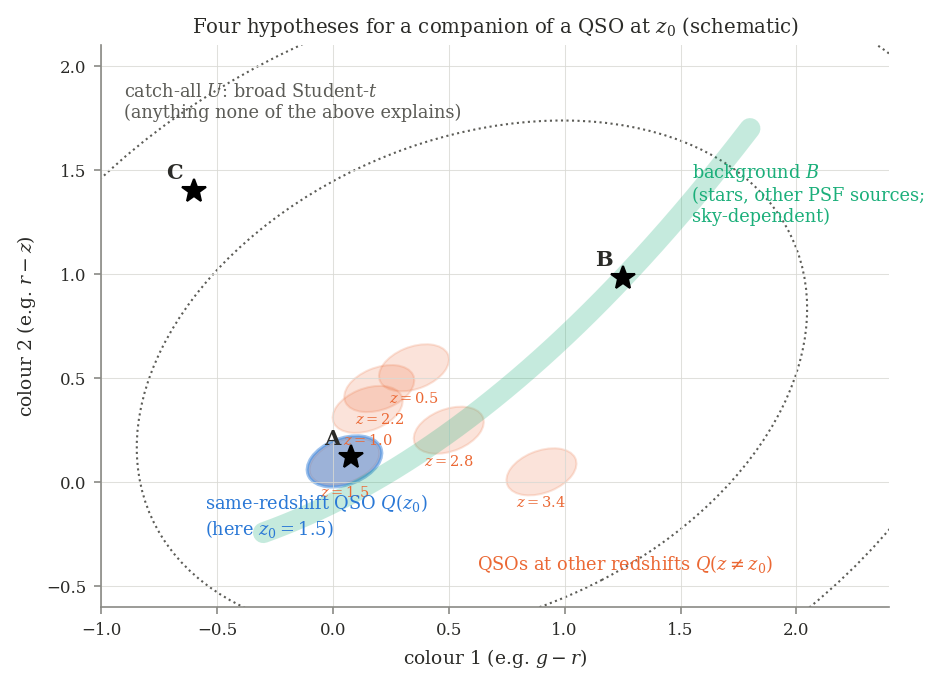
\includegraphics[width=0.72\textwidth]{F01_schematic.png}
\caption{Schematic (synthetic, not fitted) of the four hypotheses in one colour plane. Candidate A
lies on the same-redshift quasar locus, B on the background locus, and C far from both; the
catch-all explains C, so the Gaussian tail of whichever population is wider does not decide it.}
\label{fig:schematic}
\end{figure}

%======================================================================
\section{Data and roles}\label{sec:data}
%======================================================================
\paragraph{Quasars.} The training quasars are the union of DESI DR1 quasars (\code{spectype=QSO},
\code{zwarn=0}, primary) and SDSS DR16Q \citep{Lyke2020}, merged by sky position. Of 1,657,444
eligible quasars, 1,049,260 are fit or select rows. Of these, 610,503 are DESI-only, 241,808
SDSS-only, and 196,949 in both (Fig.~\ref{fig:samples}). The remaining quasars are 239,371
calibration and 368,813 test rows. Their photometry was acquired from all seven surveys and stored
as native fluxes and variances.

\paragraph{Background.} The background sample is 2,978,857 cleaned point sources in 274 sky regions
(Legacy \code{type=PSF}, mask-clean, known quasars removed), with seven-survey photometry. Of these,
1,975,894 are fit or select rows and 502,251 calibration rows.

\paragraph{Selection.} All samples satisfy $|b|\geq25^\circ$. A band is used only when its survey marks
it usable (finite flux, positive variance, a positive exposure count where reported, and the survey's
cleanliness flag); weak and negative fluxes are kept. The quasar models were trained without a
signal-to-noise cut (0.7\% of their fit/select rows lie below the faint limit). The background is
trained, and all objects are scored, only above the faint limit of Section~\ref{sec:faint}.

\paragraph{Roles.} Roles are assigned by sky region before any fitting (Fig.~\ref{fig:roles}). The
background regions are 274 cones of radius $0.3^\circ$: 146 fit, 34 select, 45 calibration and 49 test
cones, so test objects lie in separate sky regions. Rows used during development to choose stopping
points or thresholds (34,259 quasars and 2,045 background objects for the quasar fits; the stopping
and evaluation rows of the background design tests) are recorded and excluded from the tests in
Section~\ref{sec:validation}.

\subsection{The faint limit}\label{sec:faint}
We train the background on, and score, only sources with Legacy $r$ at $S/N\geq10$
($\sigma_r\lesssim0.11$\,mag; $\sigma(g-r)\approx0.2$\,mag). Below this the colour errors are as large
as the colour difference between quasars and stars, and the model cannot vouch for a quasar: on the
2 October bundles, the fraction of held-out quasars given $p_{\rm quasar}>0.5$ is 19\% at
$5\leq S/N<7$ and 30\% at $7\leq S/N<10$, against 51\% at $10\le S/N<15$ and 93\% above $S/N=50$
(Fig.~\ref{fig:snrcut}). The limit is a signal-to-noise cut rather than a magnitude cut because the
two hemispheres differ in depth: stellar counts peak at $r\approx24.6$ in the South and $r\approx23.6$ in
the North, and $S/N=10$ falls at $r\approx24.1$ and 22.9 respectively. It removes 2.8\% of test quasars
and 64\% of test background objects, almost all faint stars. Legacy $r$ is then the reference band of
every scored source, so the quasar and background densities are conditioned on the same magnitude
that defines the background bins. A source without Legacy $r$ (for example SDSS-only photometry) is
not scored; on the training samples that affects 0.01\% of quasars.

\begin{figure}[!htbp]\centering
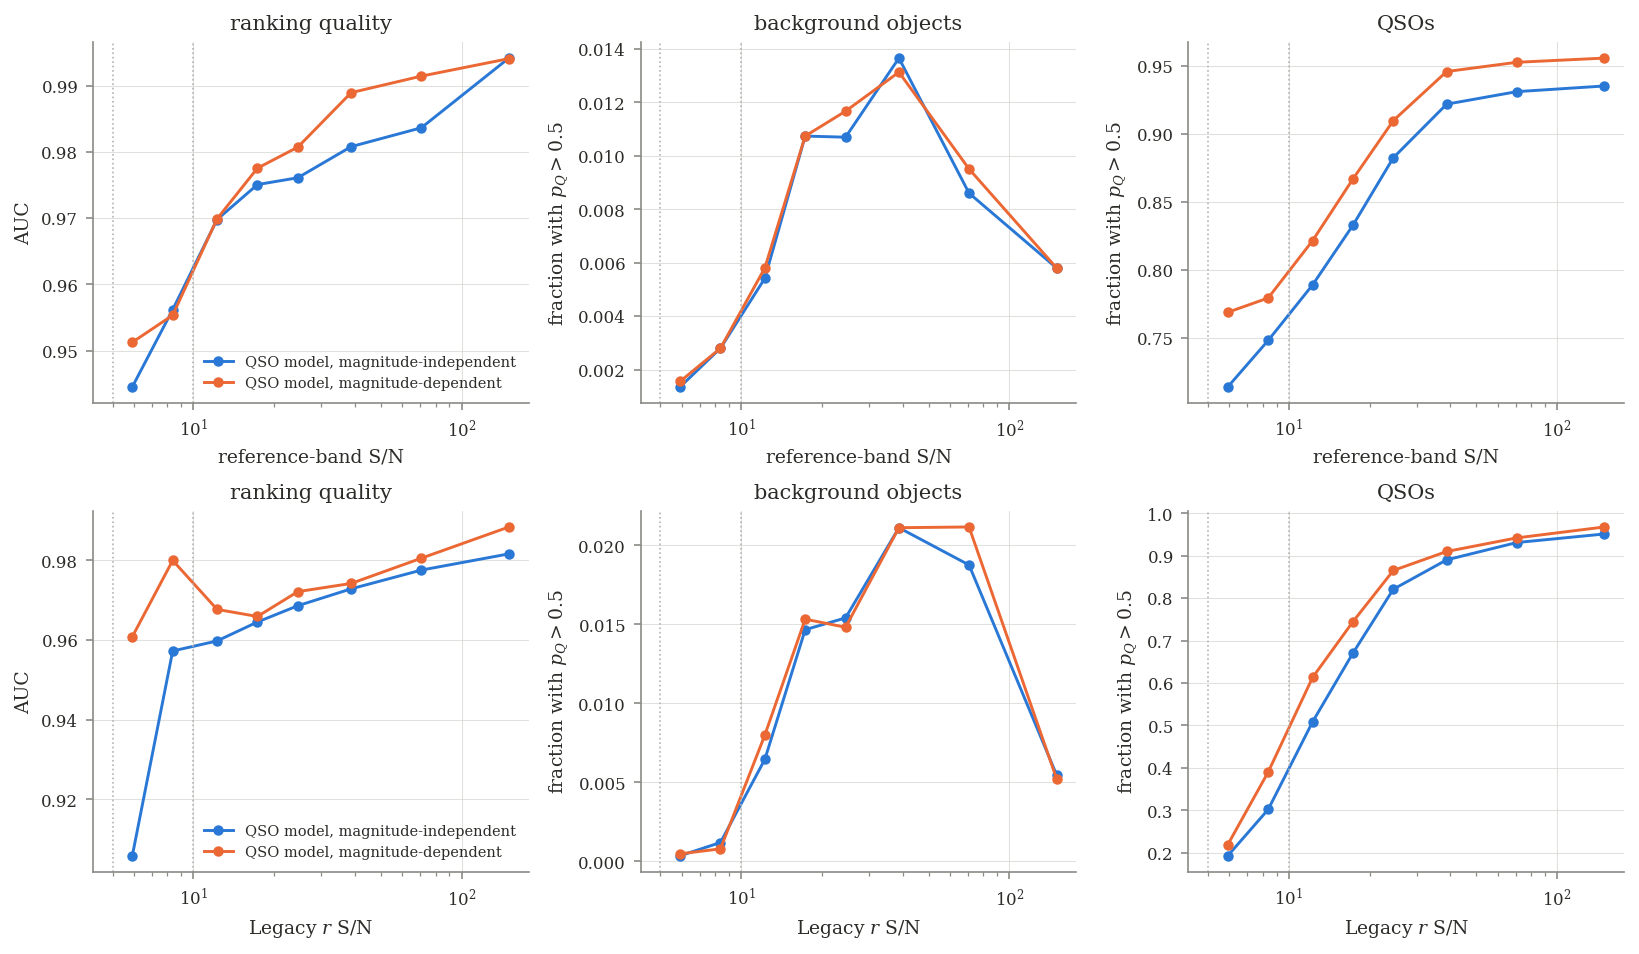
\includegraphics[width=\textwidth]{F17_snr_cut_check.png}
\caption{Held-out performance of the 2 October bundles against signal-to-noise, before the faint limit.
Top: S/N of the band then used as reference (SDSS $r$ first). Bottom: S/N of Legacy $r$. Left: AUC within
each S/N bin. Middle and right: fraction of background objects and of quasars given
$p_{\rm quasar}>0.5$. Dotted lines: $S/N=5$ and 10.}
\label{fig:snrcut}
\end{figure}

\begin{figure}[!htbp]\centering
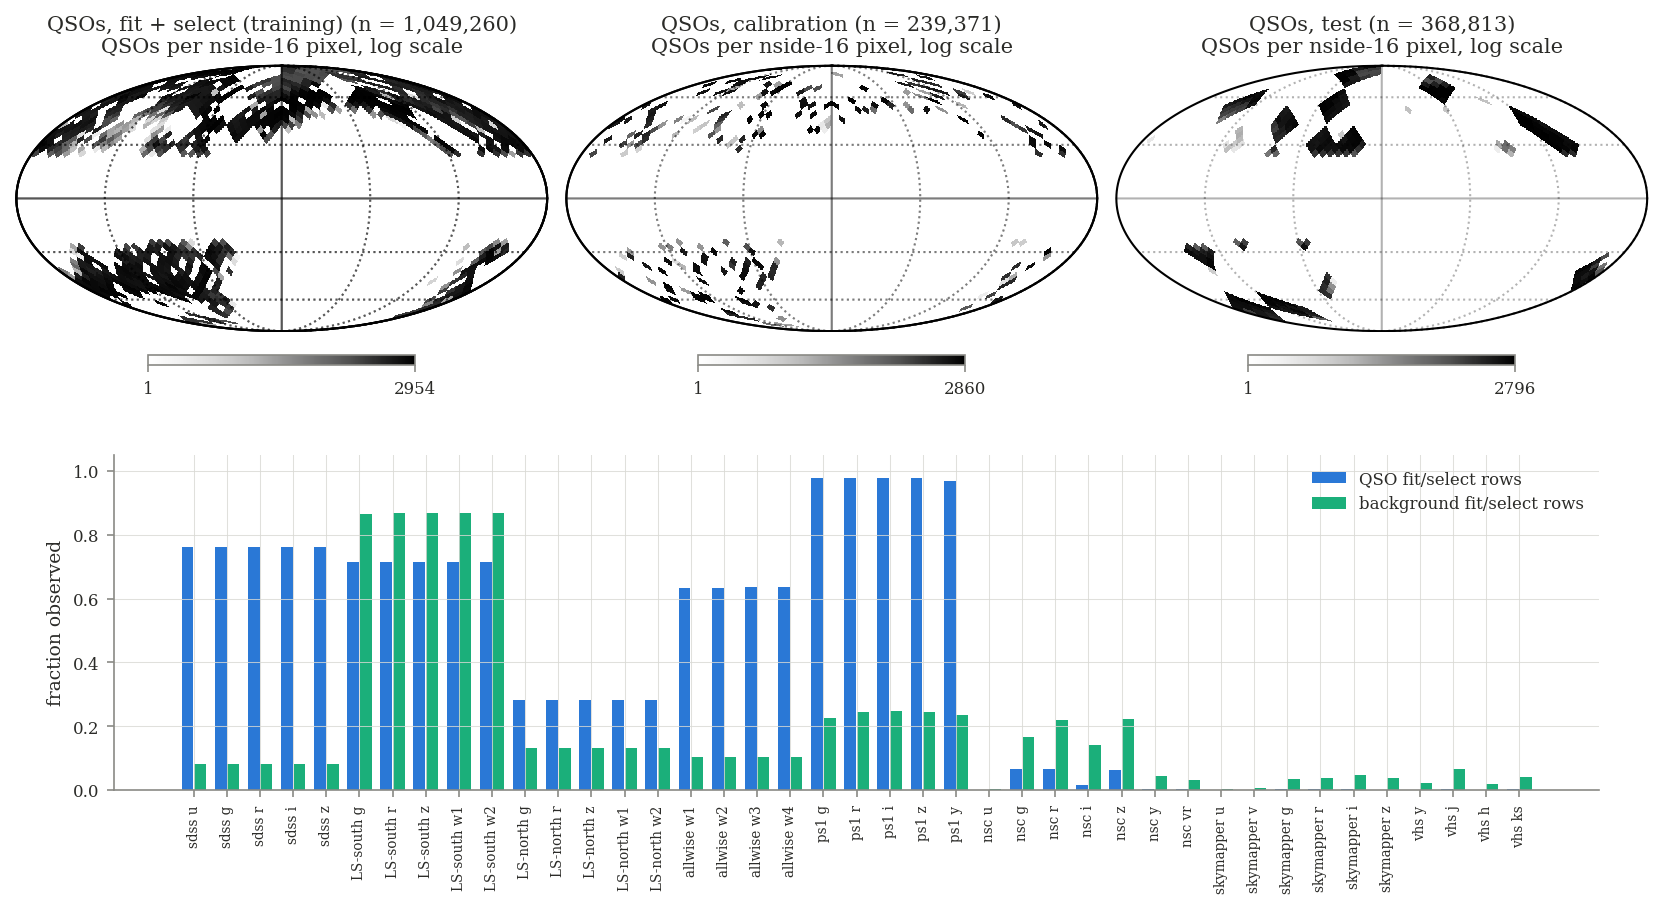
\includegraphics[width=\textwidth]{F02_data_roles_bands.png}
\caption{Top: sky distribution of quasars by role, Galactic Mollweide projection, counts per HEALPix
nside-16 pixel (log scale). Bottom: fraction of fit/select rows with each band observed, for quasars
(blue) and the background (aqua).}
\label{fig:roles}
\end{figure}

\begin{figure}[!htbp]\centering
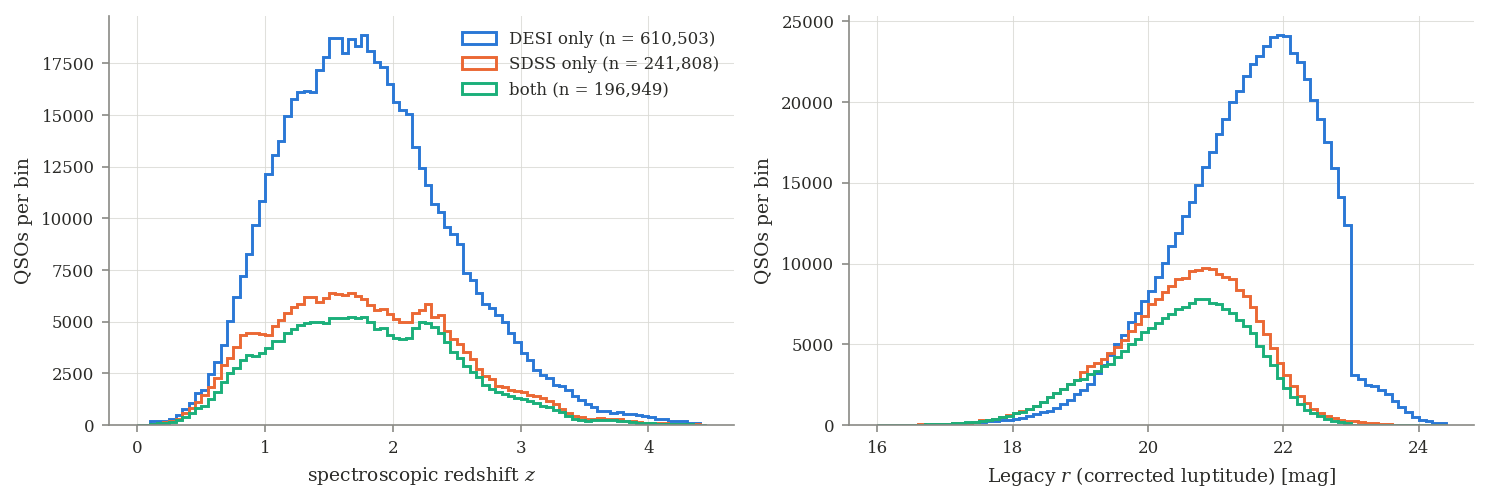
\includegraphics[width=\textwidth]{F03_qso_samples.png}
\caption{Fit/select quasars by parent survey. Left: spectroscopic redshift. Right: Legacy $r$
(extinction-corrected luptitude, southern band where observed, otherwise northern). The DESI-only
sample ends near DESI's quasar target limit, $r\approx23$.}
\label{fig:samples}
\end{figure}

%======================================================================
\section{Photometry and the observation model}\label{sec:photometry}
%======================================================================
\subsection{Native luptitudes and measurement errors}
Every band keeps its native calibration and zero point (AB for SDSS, Legacy, PS1, NSC and SkyMapper;
Vega for AllWISE and VHS). Fluxes become luptitudes with a per-band softening $s$, and their
variances propagate through the exact derivative of the luptitude function. A band that is not
observed is marginalised exactly; it is never imputed.

\subsection{Galactic extinction}\label{sec:extinction}
Fluxes and variances are corrected before any other step:
\begin{equation}
f\rightarrow f\,10^{0.4R_jE},\qquad \sigma_f^2\rightarrow\sigma_f^2\,10^{0.8R_jE},
\end{equation}
where $E$ is the SFD98 reddening \citep{SFD98} at the source position. This preserves signal-to-noise
and keeps negative fluxes negative. Table~\ref{tab:ext} lists the coefficients. Legacy DR9 values come
from the survey documentation \citep{LSDR9}, SDSS and PS1 values from \citet{SF11}, Table~6, and
SkyMapper values from \citet{Wolf2018}. NSC $VR$ and VHS $Y$ have no published values in these sources.
We computed them with the \citet{SF11} method: an F99 law with $R_V=3.1$ and a 7000\,K source, with
one scale factor fitted to 16 published rows (residual rms 0.73\%). Top-hat bandpasses were used,
so these two values are approximate; we estimate $\pm5\%$ for $VR$. The scorer computes $E$ from
the candidate's position and applies the same correction, so users supply catalogue fluxes as
observed. Fig.~\ref{fig:extinction} shows that our correction reproduces the Legacy catalogue
correction (\code{mw\_transmission}) to 0.002\,mmag.

\begin{table}[!htbp]\centering\small
\caption{Extinction coefficients $R_j=A_j/E(B-V)_{\rm SFD}$.}\label{tab:ext}
\begin{tabular}{p{0.27\textwidth}p{0.33\textwidth}p{0.32\textwidth}}
\toprule
Bands & $R_j$ & Source \\
\midrule
Legacy DECam $g,r,z$ & 3.214, 2.165, 1.211 & Legacy DR9 documentation \\
Legacy North $g,r,z$ & 3.278, 2.189, 1.196 & DECam values through the DESI relation, Eq.~(\ref{eq:Rnorth}) \\
$W1,W2$ (Legacy, AllWISE); $W3,W4$ & 0.184, 0.113; 0.0241, 0.00910 & Legacy DR9 documentation \\
SDSS $ugriz$ & 4.239, 3.303, 2.285, 1.698, 1.263 & \citet{SF11}, $R_V=3.1$ \\
PS1 $grizy$ & 3.172, 2.271, 1.682, 1.322, 1.087 & \citet{SF11} \\
NSC $ugrizY$ & 3.995, 3.214, 2.165, 1.592, 1.211, 1.064 & DECam (Legacy DR9) \\
NSC $VR$ & 2.28 & computed, approximate \\
SkyMapper $uvgriz$ & 4.294, 4.026, 2.986, 2.288, 1.588, 1.206 & \citet{Wolf2018} \\
VHS $J,H,K_s$; $Y$ & 0.709, 0.449, 0.302; 1.00 & UKIRT rows of \citet{SF11}; $Y$ computed \\
\bottomrule
\end{tabular}
\end{table}

\begin{figure}[!htbp]\centering
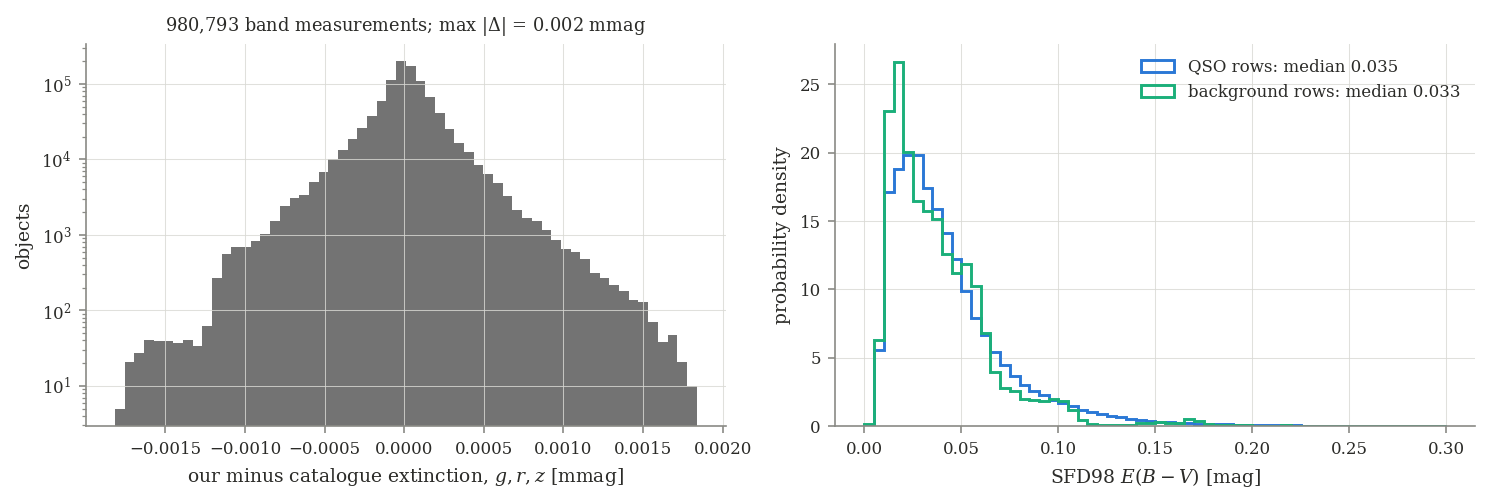
\includegraphics[width=\textwidth]{F04_extinction.png}
\caption{Left: our correction minus the Legacy catalogue correction, in four reserved Legacy cones
(980,793 $g,r,z$ measurements). Right: distribution of SFD98 reddening for the quasar and background
rows (medians 0.035 and 0.033\,mag).}
\label{fig:extinction}
\end{figure}

\subsection{One latent model for Legacy North and South}\label{sec:latent}
Legacy DR9 South (DECam) and North (BASS/MzLS) $g,r,z$ use different filters. Earlier models fitted
them as separate bands, and the northern fits then borrowed little from the much larger southern
sample. We now describe every source by latent, noise-free luptitudes $\vect{x}$ in 36 coordinates:
five shared Legacy coordinates (\code{legacy:g,r,z,W1,W2}) and 31 coordinates for the other surveys.
The 41 native bands follow from a linear operator,
\begin{equation}
\vect{y}=H\vect{x}+\vect{b}+\vect{\epsilon},\qquad \vect{\epsilon}\sim N(0,T).
\end{equation}
Rows of $H$ for the southern Legacy and all non-Legacy bands are unit vectors. Rows for the
northern $g,r,z$ carry the DESI North$\to$South colour relation. For example,
$y_{g,N}=1.0627\,x_g-0.0643\,x_r+0.0016\,x_z-0.0060$. $T$ holds the instrumental scatter measured
on overlap pairs. The relation acts on uncorrected magnitudes, so extinction is removed in the DECam
system:
\begin{equation}\label{eq:Rnorth}
R_{\rm native}=H\,R_{\rm latent},
\end{equation}
where each latent coordinate takes the coefficient of the system it represents. Fig.~\ref{fig:northsouth}
shows that the relation removes the colour-dependent North--South offsets on the same objects. The
Legacy $W1,W2$ coordinates are shared after both hemispheres use common units and softening; they
remain distinct from AllWISE $W1,W2$.

\begin{figure}[!htbp]\centering
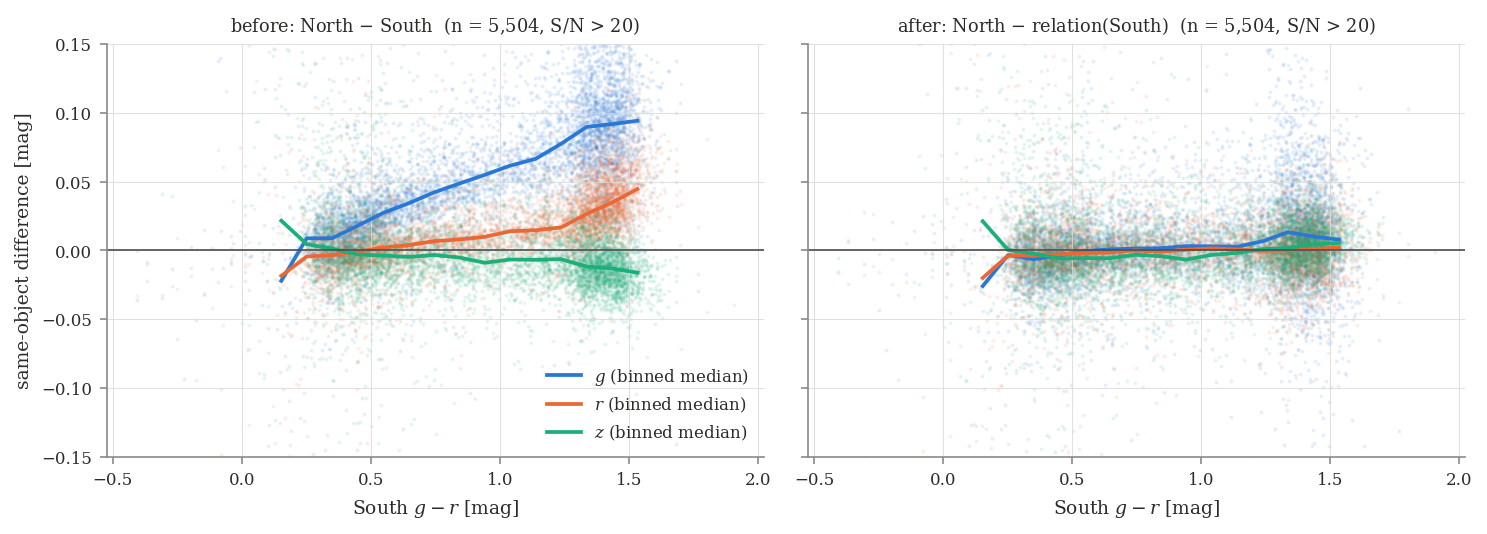
\includegraphics[width=\textwidth]{F05_north_south.png}
\caption{Same-object North minus South luptitudes in overlap fields ($S/N>20$ in all six bands),
against South $g-r$. Left: raw difference. Right: after applying the DESI relation to the southern
values. Lines: binned medians.}
\label{fig:northsouth}
\end{figure}

%======================================================================
\section{The quasar model}\label{sec:qso}
%======================================================================
\subsection{Redshift slices and extreme deconvolution}
For each of the 43 slices, the latent quasar luptitudes follow a Gaussian mixture with $K$
components ($K=20$ for 23 slices, 12 for 6, 8 for 13, and 4 for the sparsest one, 640 objects at
$z=4.35$):
\begin{equation}
p(\vect{x}\mid Q,z_k)=\sum_{i=1}^{K}\alpha_i\,N(\vect{x};\vect{\mu}_i,V_i).
\end{equation}
Extreme deconvolution \citep{Bovy2011XD} fits $\alpha_i,\vect{\mu}_i,V_i$ to noisy, incomplete data.
Each object contributes $N(\vect{y};H\vect{\mu}_i+\vect{b},HV_iH^{\rm T}+T+\vect{C})$ in its observed
bands only, so measurement errors are removed from the fitted widths rather than absorbed into them.
Section~\ref{sec:fitting} describes the fitting. At scoring time the candidate's own covariance is
added back, and the density is conditioned on the reference band:
$p(\vect{y}_{\rm other}\mid m_{\rm ref})=p(\vect{y})/p(m_{\rm ref})$. The scorer interpolates linearly
between neighbouring slices in redshift.

\subsection{Two variants: with and without magnitude dependence}\label{sec:variants}
Conditioning a joint mixture on $m_{\rm ref}$ lets a model's colour distribution depend on apparent
magnitude: a component's colour mean shifts with $m_{\rm ref}$ unless its covariance forbids it. The
XDQSO design \citep{Bovy2011XDQSO} forbids it, and leaves all magnitude dependence to the abundance
prior $\Sigma_Q(z,m)$. We provide both:

\paragraph{Magnitude-independent (default).} We rewrite the latent vector as one magnitude and 35 colours,
$u_r=x_r$ and $u_j=x_j-x_r$ for $j\neq r$, with $r$ the shared Legacy $r$ coordinate. In every component
the magnitude coordinate has the same fixed distribution, $N(20,100\,{\rm mag}^2)$, and zero
covariance with the colours. Conditioning on any reference band then leaves the colour likelihood
independent of brightness. The residual dependence through the finite magnitude variance is below
$10^{-3}$\,nat for a $\pm3$\,mag shift. With this block structure the likelihood factorises, and the
exact constrained M step is the ordinary update of the colour block. A unit test confirms that it
equals a fit to the colours alone.

\paragraph{Magnitude-dependent.} The same mixture without the constraint.

\paragraph{Why both are kept.} DESI and SDSS selected their quasars with colour cuts that change with
magnitude. A model allowed to depend on magnitude can learn that selection as if it were quasar
physics, and then penalise genuine quasars outside the selection. The test quasars share the training
selection, so our tests cannot measure this risk. They can measure the cost of the constraint, which
Section~\ref{sec:validation} reports.

\begin{figure}[!htbp]\centering
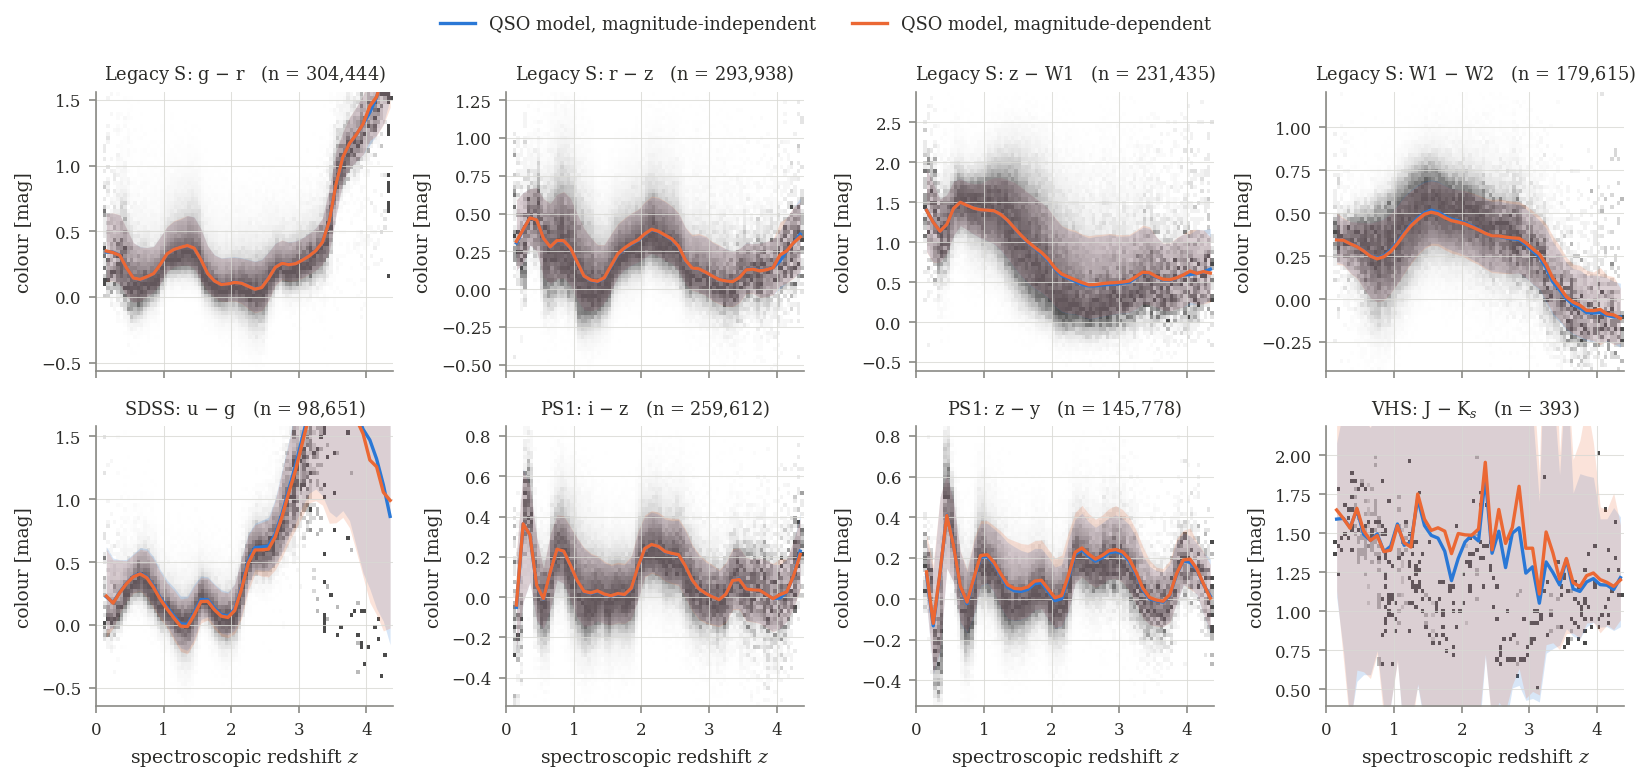
\includegraphics[width=\textwidth]{F06_colour_redshift.png}
\caption{Quasar colour against redshift. Grey: test quasars with both bands at $S/N>10$ (density
normalised in each redshift column of width 0.05). Lines and bands: per-slice median and 16--84\% range
of the noise-free model colour, magnitude-independent (blue) and magnitude-dependent (orange, marginalised
over magnitude). The data include measurement noise and a signal-to-noise selection that the model
bands do not.}
\label{fig:colourz}
\end{figure}

%======================================================================
\section{The background model}\label{sec:background}
%======================================================================
\paragraph{Why the design changed.} The 2 October background was one $K=20$ mixture over all
magnitudes. Faint sources dominate the training counts (69\% of fit/select rows had $r>23.5$), so
nearly all components described faint objects, and bright stars were covered by about one broad
component: at $17\le r<19$, half of that model's draws fell in empty colour space, and its contours did
not follow the stellar locus (Fig.~\ref{fig:stellarfinal}, top rows). Two cheaper fixes failed in light
tests: decoupling magnitude from colour inside each component, and sharing 20 colour shapes across
magnitude nodes with only their weights free (worse than the joint model at $r>22$, so the shape of the
locus itself changes with magnitude). We therefore follow XDQSO \citep{Bovy2011XDQSO}, which fits stars
in narrow magnitude bins; CondXD \citep{Kang2025} reaches comparable results with a neural network that
makes all mixture parameters functions of magnitude.

\paragraph{Binned fit.} The fit/select background rows above the faint limit are split into eight bins of
Legacy $r$: 15.5--17, 17--18, \dots, 22--23 and 23--24.5. Each bin is fitted independently by extreme
deconvolution with $K=20$ components over the 36 latent coordinates (written as $r$ and 35 colours),
on its own rows plus those within 0.25\,mag of its edges (19,158 to 255,709 rows per bin), with the
MAP update and predictive early stopping of Section~\ref{sec:fitting} on 1,000 test-role objects per
bin. The eight mixtures are joined into one 160-component mixture, each bin's weights scaled by its
share of training objects. Conditioning this mixture on $m_{\rm ref}$ weights each component by
$N(m_{\rm ref};\mu_{r,i},V_{rr,i})$, which selects the bin and blends neighbouring bins smoothly at the
edges; on held-out stars this is $0.1$--$0.3$\,nat better than picking one bin. Because $m_{\rm ref}$ is
Legacy $r$ for every scored source, routing and conditioning use the same magnitude.

\paragraph{Training sample cleaned of quasars.} Known quasars (DESI DR1, DR16Q) were removed from the
background sample when it was built, but it still contains unidentified ones, increasingly at faint
magnitudes: among background rows detected in $W1$ and $W2$, the fraction with the AGN colour
$W1-W2>0.8$ (Vega; \citealt{Stern2012}) is 3\% at $19\le r<20$ and 37\% at $22\le r<23$. A binned model
is flexible enough to learn them as background, which lowered the recall of real quasars in a light
test (0.83 to 0.74). We therefore remove from training (and from the background test sets) members of
Quaia \citep{StoreyFisher2024} matched by Gaia DR3 \code{source\_id}, and sources with $W1-W2>0.8$ (Vega)
at $S/N\ge5$ in both bands, except very red optical sources ($r-z>2$, kept as brown-dwarf candidates).
This removes 0.1\% of training rows at $r<18$ and 3--5\% at $r>20$. A Gaia zero-proper-motion cut was
tested and rejected: 33--56\% of zero-motion sources have stellar $W1-W2$ even at
$\sigma_\mu<0.2$--$0.5$\,mas\,yr$^{-1}$ (distant halo stars), and Gaia does not reach the faint bins where
contamination matters. Faint unidentified quasars not detected by WISE remain; we accept this.

\paragraph{Sky dependence.} Component shapes are the same everywhere; the weights vary with position as
a softmax gate,
\begin{equation}
w_i(\ell,b)\propto\exp\!\left[a_i+\vect{\beta}_i\cdot\vect{f}(\ell,b)\right],\qquad
\vect{f}=\left(\csc|b|,\ \cos\ell,\ \sin\ell,\ \csc|b|\cos\ell,\ {\rm sign}\,b\right),
\end{equation}
fitted by maximum likelihood with fixed component densities and an L2 penalty of 1 on $\vect{\beta}$,
on 300,000 cleaned training rows. On 60,000 held-out rows in the test cones it improves the held-out
density over one all-sky weight vector by $0.0285\pm0.0014$\,nat per object, positively in every
magnitude and $|b|$ bin, and beats the previous HEALPix hierarchy (nside 4, $n_0=1000$:
$0.0207\pm0.0011$). The scorer evaluates the gate at nside-16 pixel centres ($3.7^\circ$; loss
0.0004\,nat). The effect is small because stellar colours at $|b|\ge25^\circ$ change little with position.

\paragraph{Surface density.} $\Sigma_B(m)$ is measured per reference band from counts in regions of
measured usable area, pooled with $n_0=100$, as before. A candidate-local refit of weights and density
in a declared cone is available.

\begin{table}[!htbp]\centering\small
\caption{Held-out conditional density $\ln p(\vect{y}_{\rm other}\mid r)$ of background objects (nat per object)
under the 2 October joint background and the binned background: 17,937 test-cone objects above the faint
limit, likely quasars removed, never used in fitting. Last column: fraction of objects better described
by the binned model.}\label{tab:bkgdensity}
\begin{tabular}{lrrrrr}
\toprule
Legacy $r$ & $N$ & joint & binned & difference & better \\
\midrule
15.5--17 & 437 & 30.56 & 35.42 & $+4.86\pm0.13$ & 97\% \\
17--18 & 2,500 & 25.45 & 28.80 & $+3.36\pm0.05$ & 94\% \\
18--19 & 2,500 & 21.82 & 24.61 & $+2.79\pm0.05$ & 92\% \\
19--20 & 2,500 & 17.24 & 19.64 & $+2.40\pm0.05$ & 89\% \\
20--21 & 2,500 & 11.55 & 13.19 & $+1.64\pm0.04$ & 86\% \\
21--22 & 2,500 & 5.30 & 6.00 & $+0.70\pm0.03$ & 73\% \\
22--23 & 2,500 & $-1.68$ & $-1.30$ & $+0.38\pm0.02$ & 66\% \\
23--24.5 & 2,500 & $-4.63$ & $-4.44$ & $+0.20\pm0.02$ & 59\% \\
\bottomrule
\end{tabular}
\end{table}

\begin{figure}[!htbp]\centering
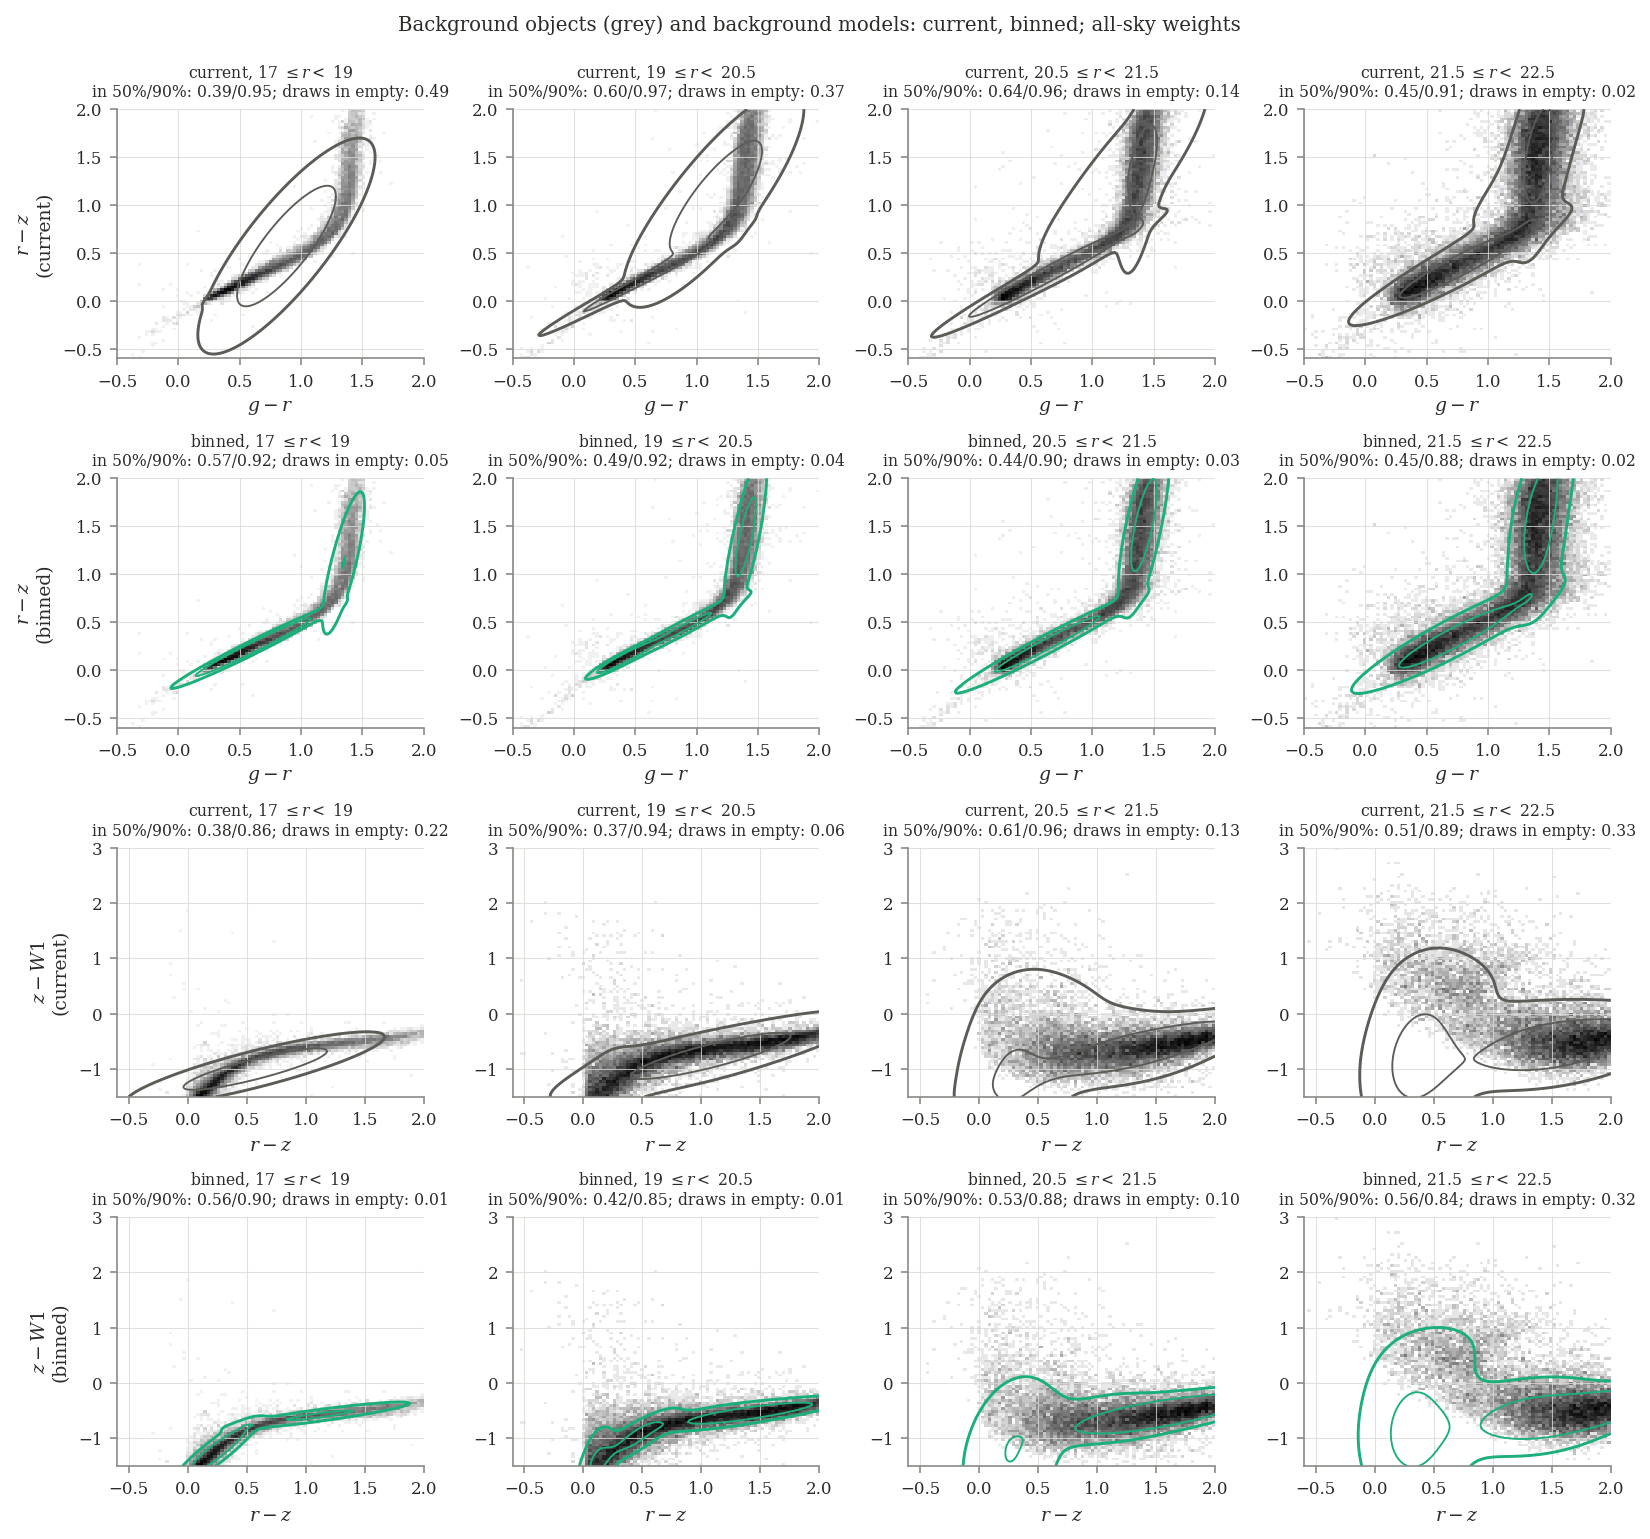
\includegraphics[width=\textwidth]{F07e_stellar_final.png}
\caption{Background objects in test cones (grey, log density) at four magnitudes, with the 2 October joint
background (grey contours) and the binned background (green), both with all-sky weights, conditioned on
the bin's central $r$ and convolved with the bin's median errors; 50\% and 90\% contours. Titles: data
fraction inside the 50\%/90\% regions and fraction of model draws in empty colour cells. In the faint
$z-W1$ panels, the plotted data require $W1$ at $S/N>5$ (46\% of stars at $21.5\le r<22.5$) while the model
describes all stars, so draws in empty cells are overstated there; Fig.~\ref{fig:stellarcc} corrects for this.}
\label{fig:stellarfinal}
\end{figure}

\begin{figure}[!htbp]\centering
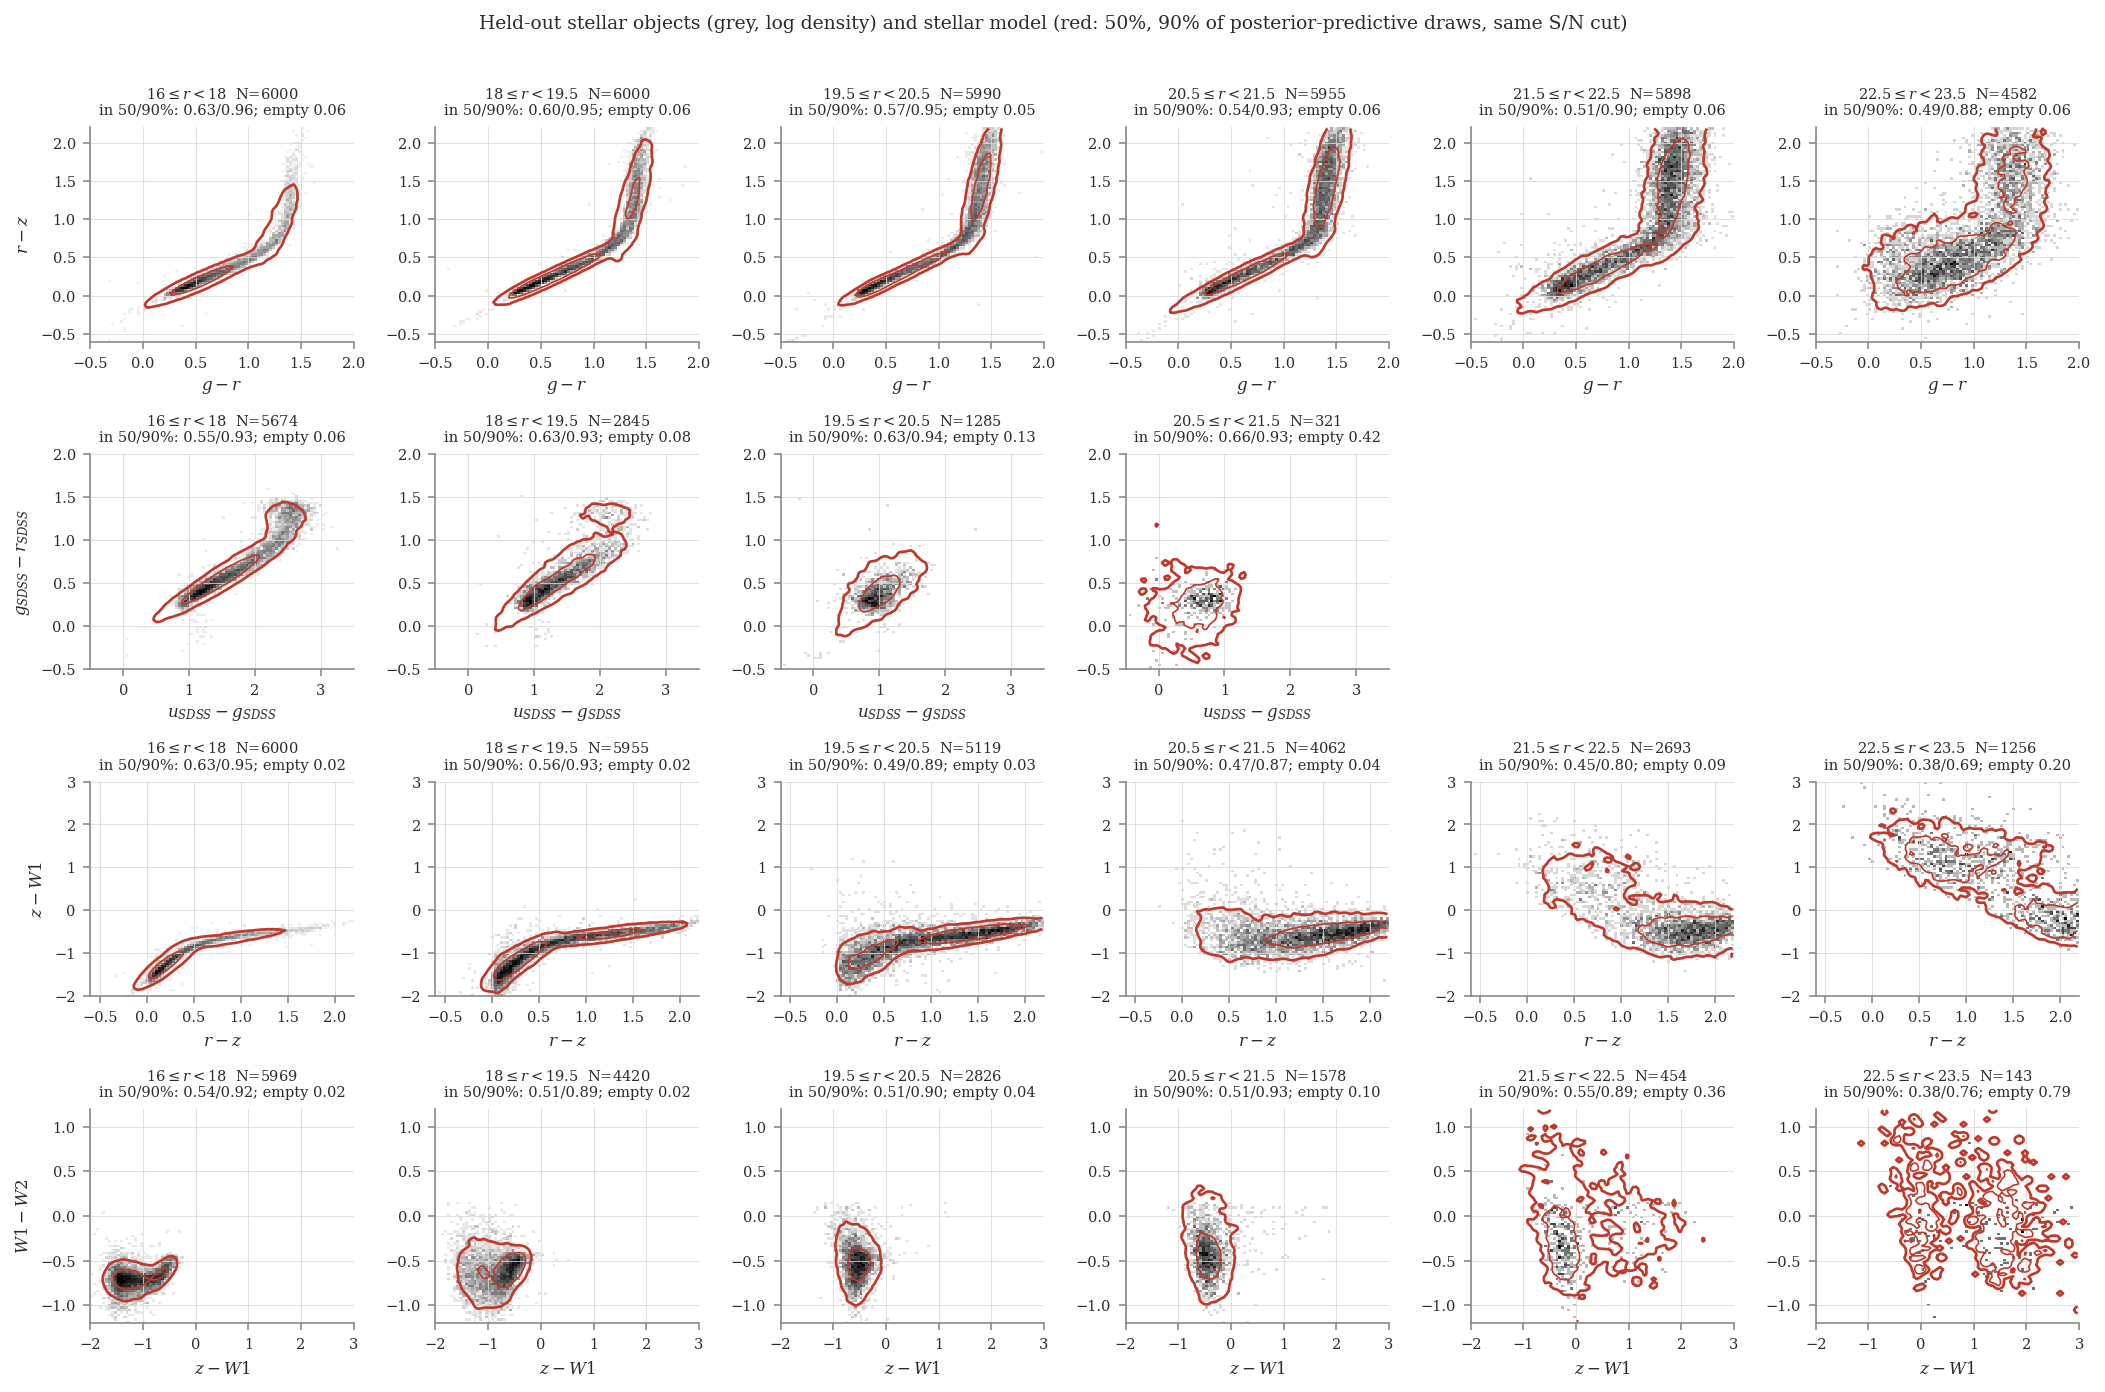
\includegraphics[width=\textwidth]{F19_stellar_colour_colour.png}
\caption{Background colour--colour density in six bins of Legacy $r$ and four planes. Grey: test-cone
background objects above the faint limit, likely quasars removed, all plane bands at $S/N\ge5$. Red:
50\% and 90\% contours of posterior-predictive draws of the binned background for the same objects
(200 per object, conditioned on each object's $r$ and sky position, with the object's own flux errors
added in flux space and the same $S/N\ge5$ selection). Titles: data inside the 50\%/90\% regions (ideal
0.50/0.90) and the fraction of draws in empty cells. Panels with fewer than 100 objects are left empty.}
\label{fig:stellarcc}
\end{figure}

%======================================================================
\section{Fitting}\label{sec:fitting}
%======================================================================
\subsection{The covariance update}
The extreme-deconvolution E step computes each component's responsibility $q_{ni}$ for object $n$, and
the posterior moments of $\vect{x}$. The M step updates the weights, the means, and the covariance from
the scatter $S_i$ about the new mean. A previous implementation used $V_i=S_i+wI$. That step maximises
no fixed objective, because its penalty is weighted by the changing responsibilities. In 24 of 43
earlier full-data quasar fits the likelihood therefore declined, by up to 0.078\,nat per object below
its best value, and a stopping rule that required a non-negative change could never stop such fits. We now use the
conjugate-prior MAP update of \citet{Bovy2011XD} (their eqs.~19--20):
\begin{equation}
V_i=\frac{q_iS_i+\nu wI}{q_i+\nu},\qquad q_i=\sum_nq_{ni},\quad \nu=1,\ w=10^{-3}\,{\rm mag}^2,
\end{equation}
which maximises the log posterior with prior $-\frac{\nu}{2}\left[\ln|V_i|+w\,{\rm tr}(V_i^{-1})\right]$
per component. EM therefore cannot decrease the reported objective (Fig.~\ref{fig:fitting}a).

\subsection{Predictive early stopping}
Every 20 updates we compute the held-out density on a fixed stopping panel: up to 512 test-role
objects per hemisphere per fit, recorded and excluded from later validation. A fit stops when a block
gains less than 0.02\,nat per object, when the objective changes by less than $10^{-4}$ (relative), or
after 300 updates. The best checkpoint, including the warm start, is kept. The 0.02\,nat threshold is
about twice the sky-bootstrap standard error of late block gains. This is predictive early stopping,
not convergence. Sparse slices benefit most: where held-out density falls in the first block, as at
$z=4.05$, the fit keeps its warm start. All 43 quasar fits of each production model stopped this way, with
no objective decrease (Fig.~\ref{fig:fitting}c,d). The eight background bins use the same rule on 1,000
test-role objects per bin, warm-started from the 2 October background with the magnitude placed at the bin
centre and equal weights; they kept checkpoints at 40--92 updates.

\begin{figure}[!htbp]\centering
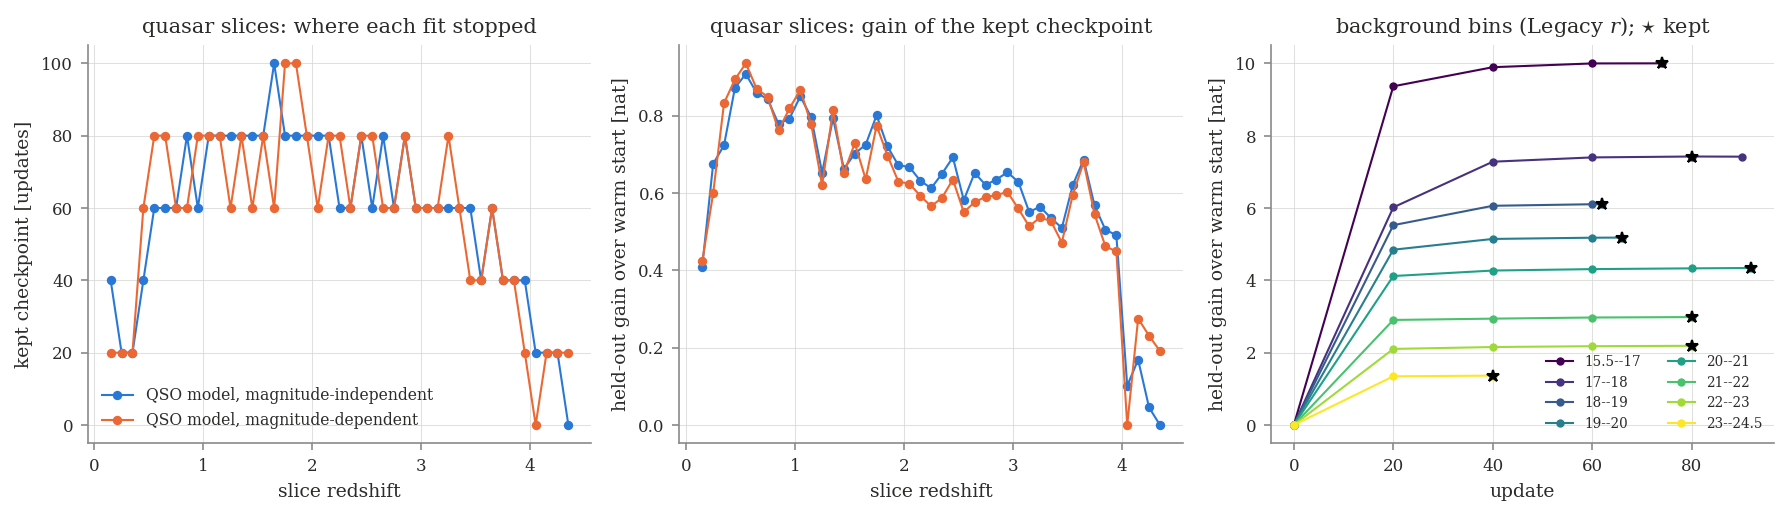
\includegraphics[width=\textwidth]{F10_fitting.png}
\caption{(a) Training objective per object minus its starting value, $z=1.75$ slice: additive
update (log likelihood; 41 decreasing steps) and MAP update (log posterior). (b) Held-out density for
six slices under both updates (identical rows and warm starts). (c) Update at which each production
fit's kept checkpoint was taken. (d) Held-out gain of that checkpoint over the model's own warm start.
The quasar fits shown are those of both bundles; the background bins are described in the text.}
\label{fig:fitting}
\end{figure}

%======================================================================
\section{Priors, catch-all and support}\label{sec:priors}
%======================================================================
\paragraph{Abundance priors.} $\Sigma_Q(z,m)$ and $\Sigma_B(m)$ are stored per reference band, per unit
native luptitude. Background densities are recounted from corrected photometry. The quasar abundance
is inherited from the previous model and moved onto corrected magnitudes by the mean extinction
shift: 0.080\,mag in Legacy $r$, at mean $E=0.037$. This is an approximation, not a recount.

\paragraph{Catch-all.} $U$ is a Student-$t$ with $\nu=4$ degrees of freedom, centred on the background
mean, with the binned background mixture's second-moment matrix as its scale. Measurement noise is
convolved exactly through the $t$'s Gaussian scale-mixture representation. Its share $\eta$ is a
Beta-MAP fit per reference band and three magnitude bins, on 148,853 calibration background objects
above the faint limit with likely quasars removed. The global share is 0.14\%, against 0.06\% for the
joint background, as expected for a tighter background model.

\paragraph{Support cut.} For a candidate, $z_0$ and the observed bands, the scorer draws 255 simulated
quasars from the conditional model at $z_0$, adds the candidate's errors, and ranks the candidate's
conditional density among them. Candidates below a threshold are not ranked; their likelihoods are
kept as diagnostics. The percentile depends on the reference band, so the threshold was recalibrated
under the faint limit on 2,000 calibration quasars (all bands and Legacy $g,r,z$ only; 3,890
evaluations). At the 99.5\% target it is again $2/256=0.0078$, retaining 99.64\% and 99.59\% of
calibration evaluations. Fig.~\ref{fig:supportcut} shows the trade-off on held-out rows: the cut at
$2/256$ removes 11 of 12 (magnitude-independent) and 3 of 3 (magnitude-dependent) high-quasar points on
artificial grids at a cost of 0.5\% of test quasars, and raises the AUC of $p_{\rm quasar}$; stricter cuts
lose quasars faster than they gain.

\begin{figure}[!htbp]\centering
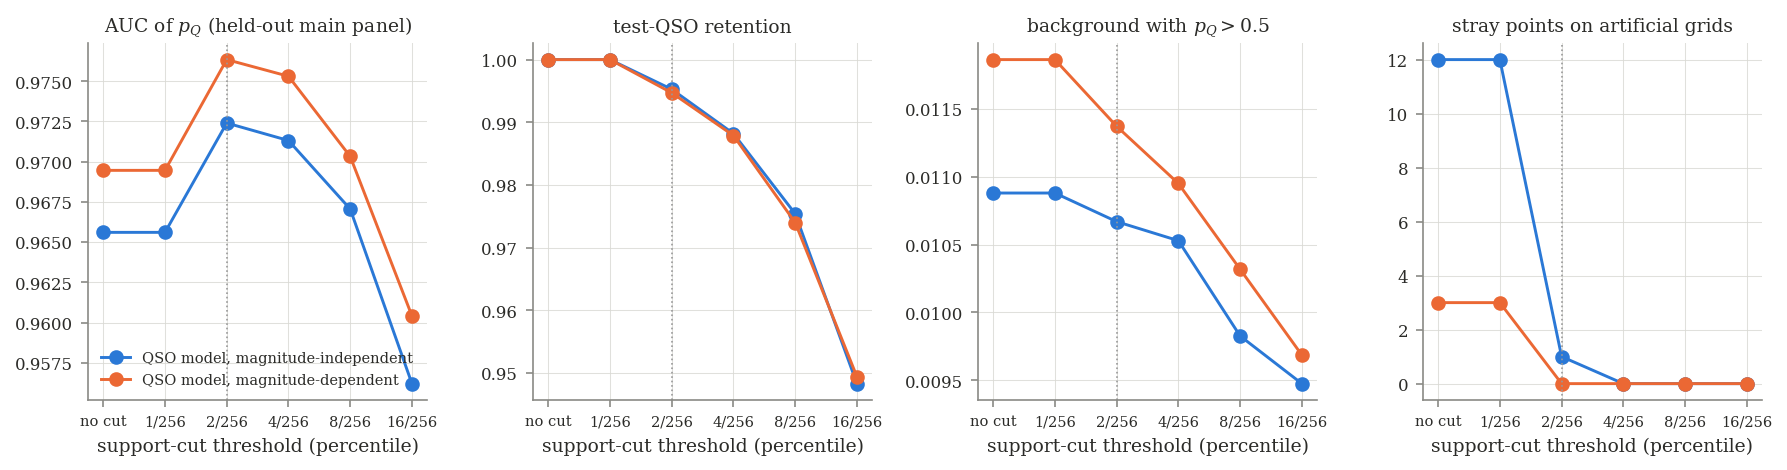
\includegraphics[width=\textwidth]{F11_support_cut.png}
\caption{Support-cut threshold (percentile; dotted: the calibrated $2/256$) on the held-out main panels of
Section~\ref{sec:perf} and the artificial grids of Section~\ref{sec:grids}: AUC of $p_{\rm quasar}$ (the
scorer does not compute $\log\R$ for rejected objects, so $p_{\rm quasar}$ ranks all thresholds alike;
unranked objects at the bottom), fraction of test quasars kept, fraction of background objects with
$p_{\rm quasar}>0.5$, and grid points with $p_{\rm quasar}>0.5$ in the low-density mask.}
\label{fig:supportcut}
\end{figure}

%======================================================================
\section{Validation}\label{sec:validation}
%======================================================================
Tests use test-role objects above the faint limit and outside every recorded development exclusion.
``Promoted'' denotes the 2 October bundles scored with the same faint limit; ``previous'' the 28 September
model.

\subsection{Colour--colour distributions}\label{sec:cc}
Figures~\ref{fig:ccmag}--\ref{fig:ccz} compare model densities with the data in two colour planes:
Legacy South $(g-r,r-z)$ and $(r-z,z-W1)$. Model contours are conditioned on each bin's median $r$,
weighted by the data's redshift mix, and convolved with the bin's median measurement covariance, so
they can be compared directly with the data. Each panel title gives the fraction of the data inside the
model's 50\% and 90\% regions; a well-calibrated model gives 0.50 and 0.90. The magnitude-dependent
quasar model gives 0.48--0.51 and 0.89--0.90 in every magnitude bin and both planes. The
magnitude-independent model must use one width for all magnitudes. It is too broad for bright
quasars (0.62/0.94 at $17\le r<19$) and too narrow for faint ones (0.41/0.86 at $21.5\le r<22.5$). The
apparent colour scatter of quasars, after deconvolution, grows towards faint magnitudes in this sample.
Underestimated photometric errors, a change in the population, and selection can all produce this.
The binned background follows the stellar locus at every magnitude and sky position: in $(g-r,r-z)$ it
gives 0.43--0.51 and 0.89--0.92 in the magnitude bins and 0.42--0.46 and 0.89--0.90 in the sky bins. In
$(r-z,z-W1)$ the 90\% coverage is 0.82--0.88; part of this is the $W1$ detection selection of the plotted
data, which Fig.~\ref{fig:stellarcc} reproduces in the model and which brings the coverage to
0.87--0.95 for $r<21.5$.

\begin{figure}[!htbp]\centering
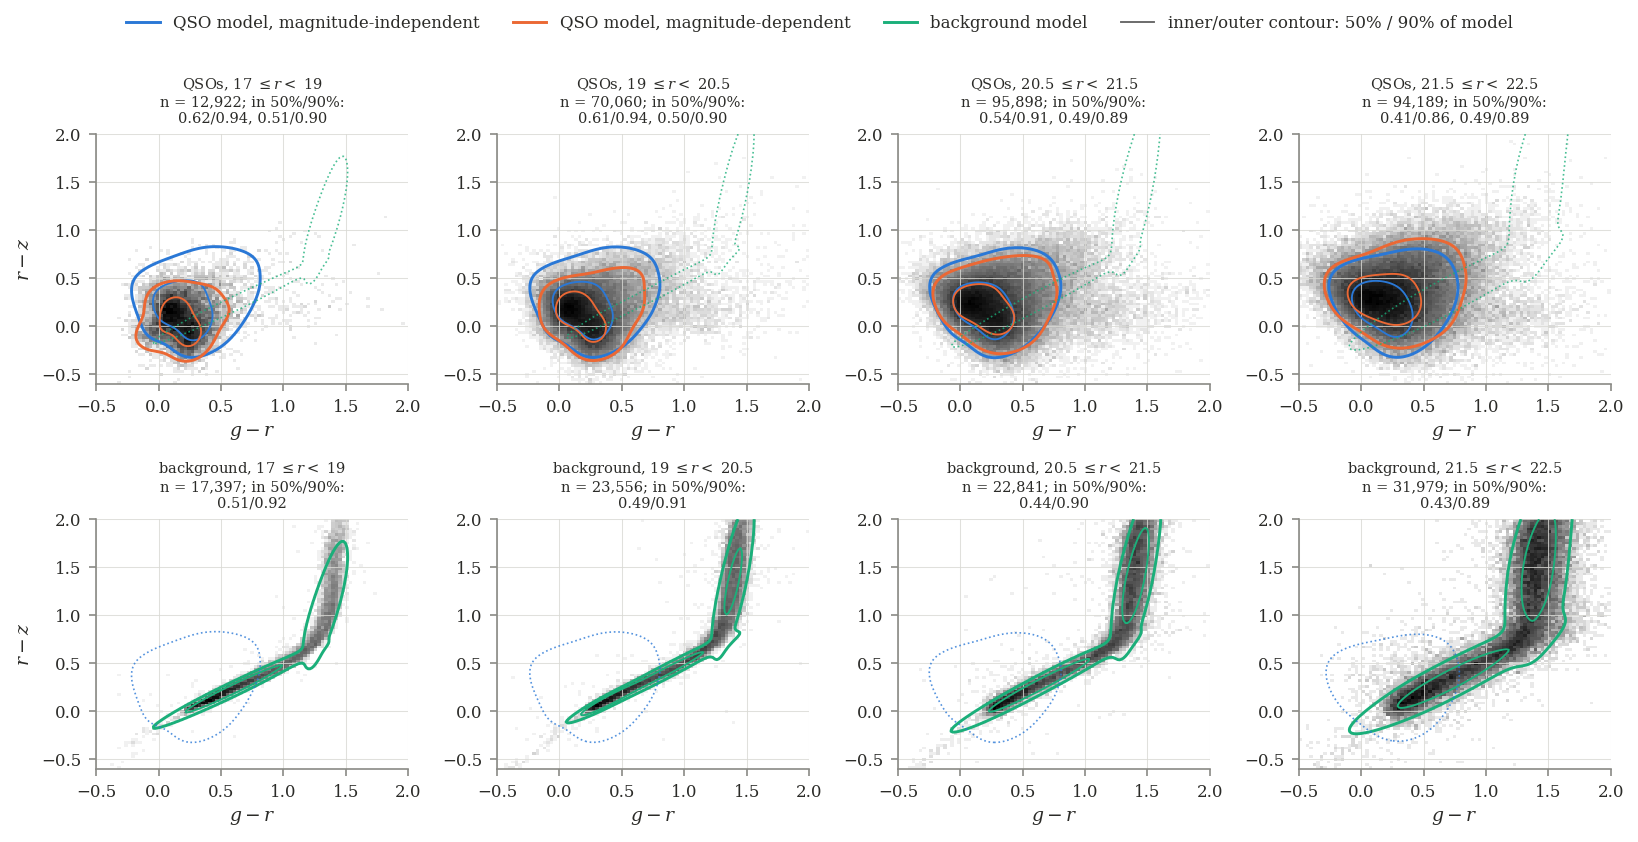
\includegraphics[width=\textwidth]{F07a_colour_colour_magnitude.png}\\[2mm]
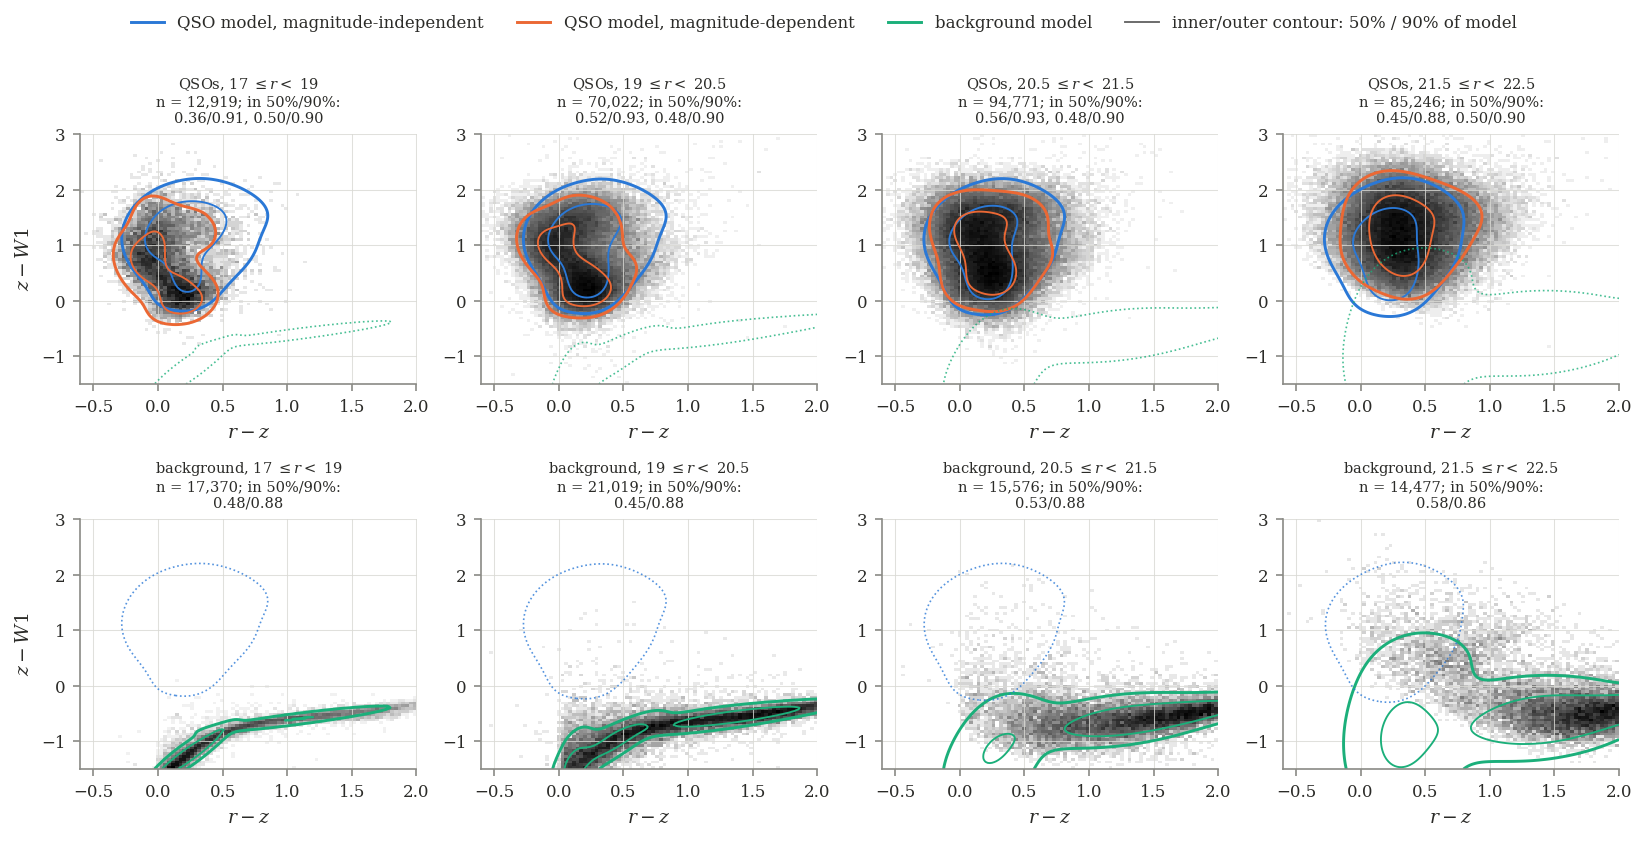
\includegraphics[width=\textwidth]{F07b_colour_colour_magnitude.png}
\caption{Colour--colour planes in bins of Legacy South $r$, objects above the faint limit. Top rows of each
block: test quasars (grey, log density) with both quasar models (blue, orange; thick and thin contours
enclose 90\% and 50\%) and the background model's 90\% contour (dotted aqua). Bottom rows: test background
objects (likely quasars removed) with the binned background and the magnitude-independent quasar model's
90\% contour (dotted blue).}
\label{fig:ccmag}
\end{figure}

\begin{figure}[!htbp]\centering
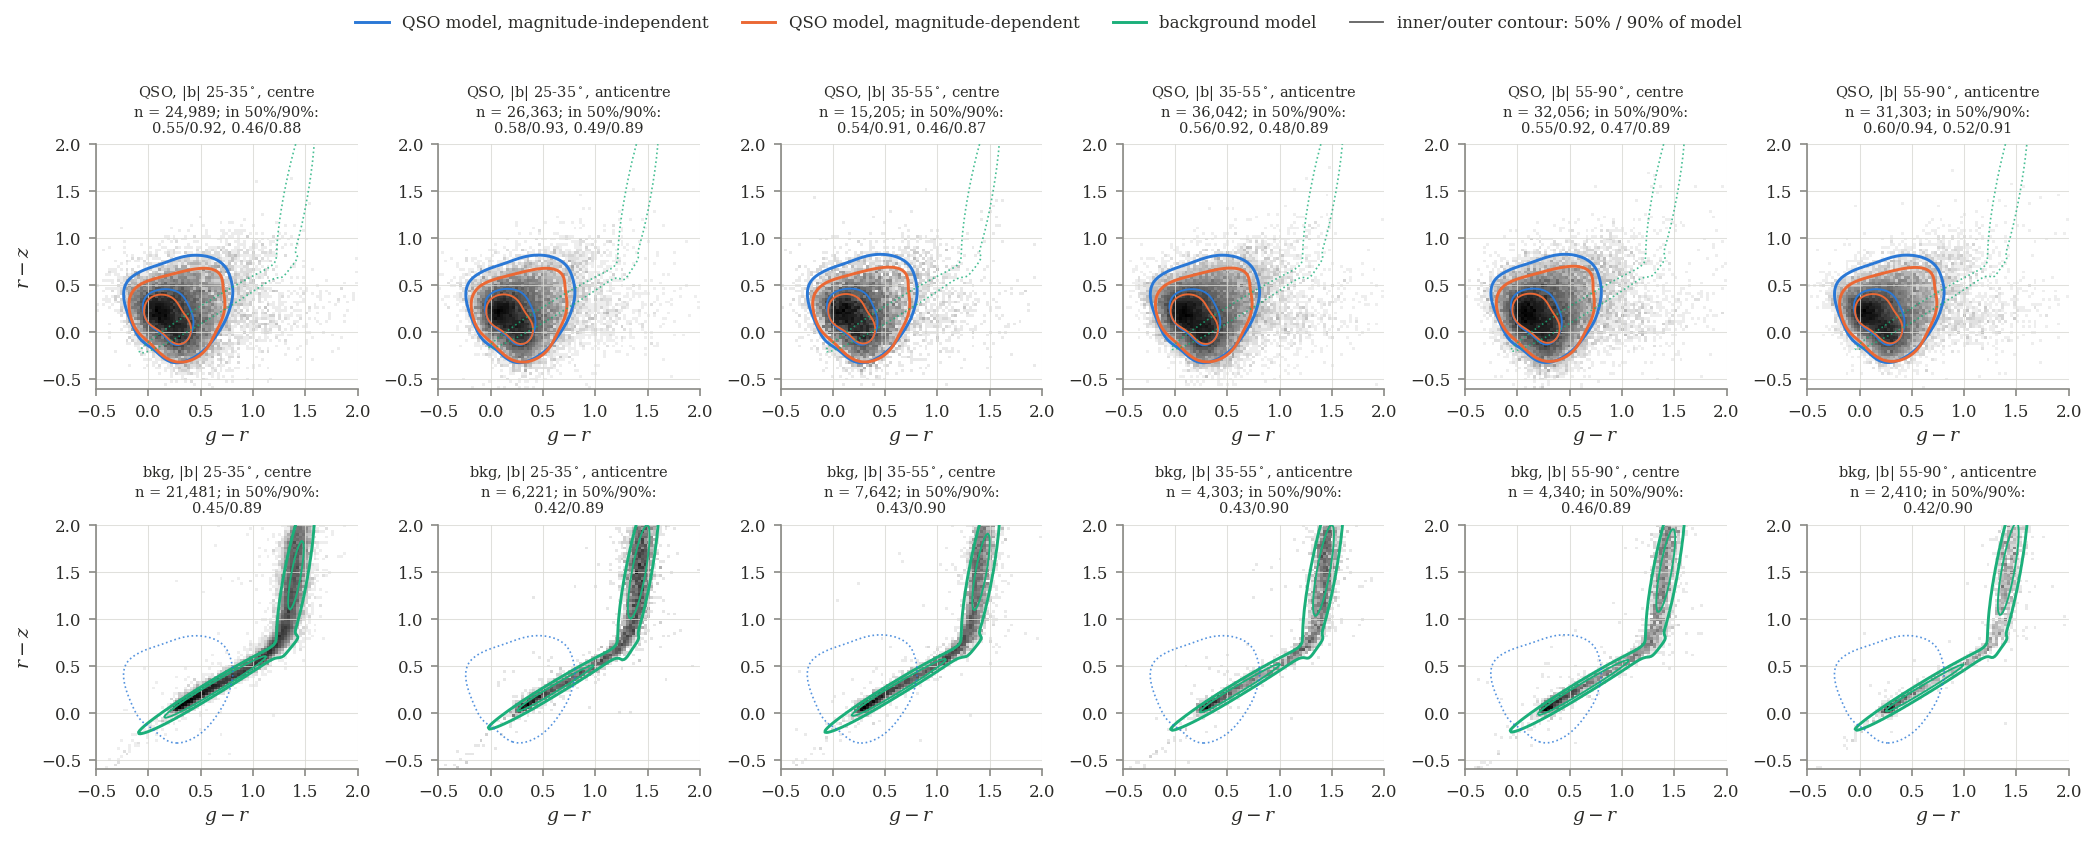
\includegraphics[width=\textwidth]{F08a_colour_colour_sky.png}\\[2mm]
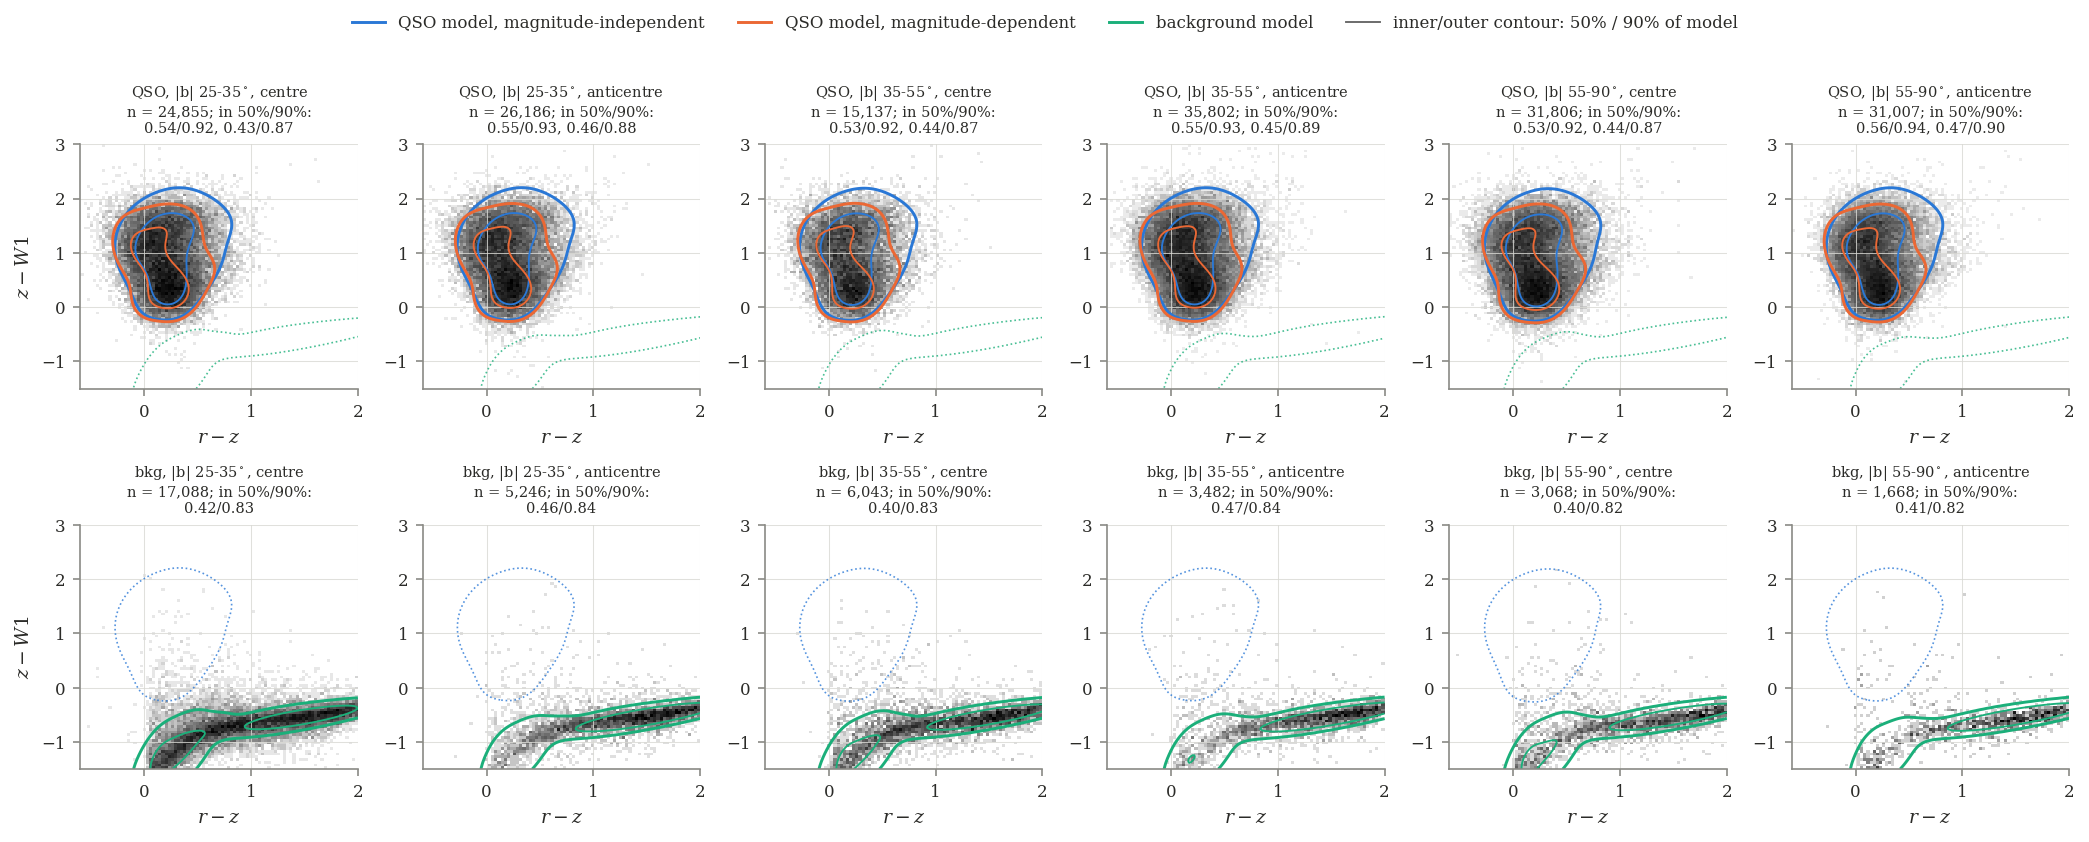
\includegraphics[width=\textwidth]{F08b_colour_colour_sky.png}
\caption{As Fig.~\ref{fig:ccmag}, in bins of Galactic latitude and of longitude towards
($|\ell|<90^\circ$) or away from the Galactic centre, at $19\le r<21.5$. Background contours use the
spatial component weights averaged over each bin's objects.}
\label{fig:ccsky}
\end{figure}

\begin{figure}[!htbp]\centering
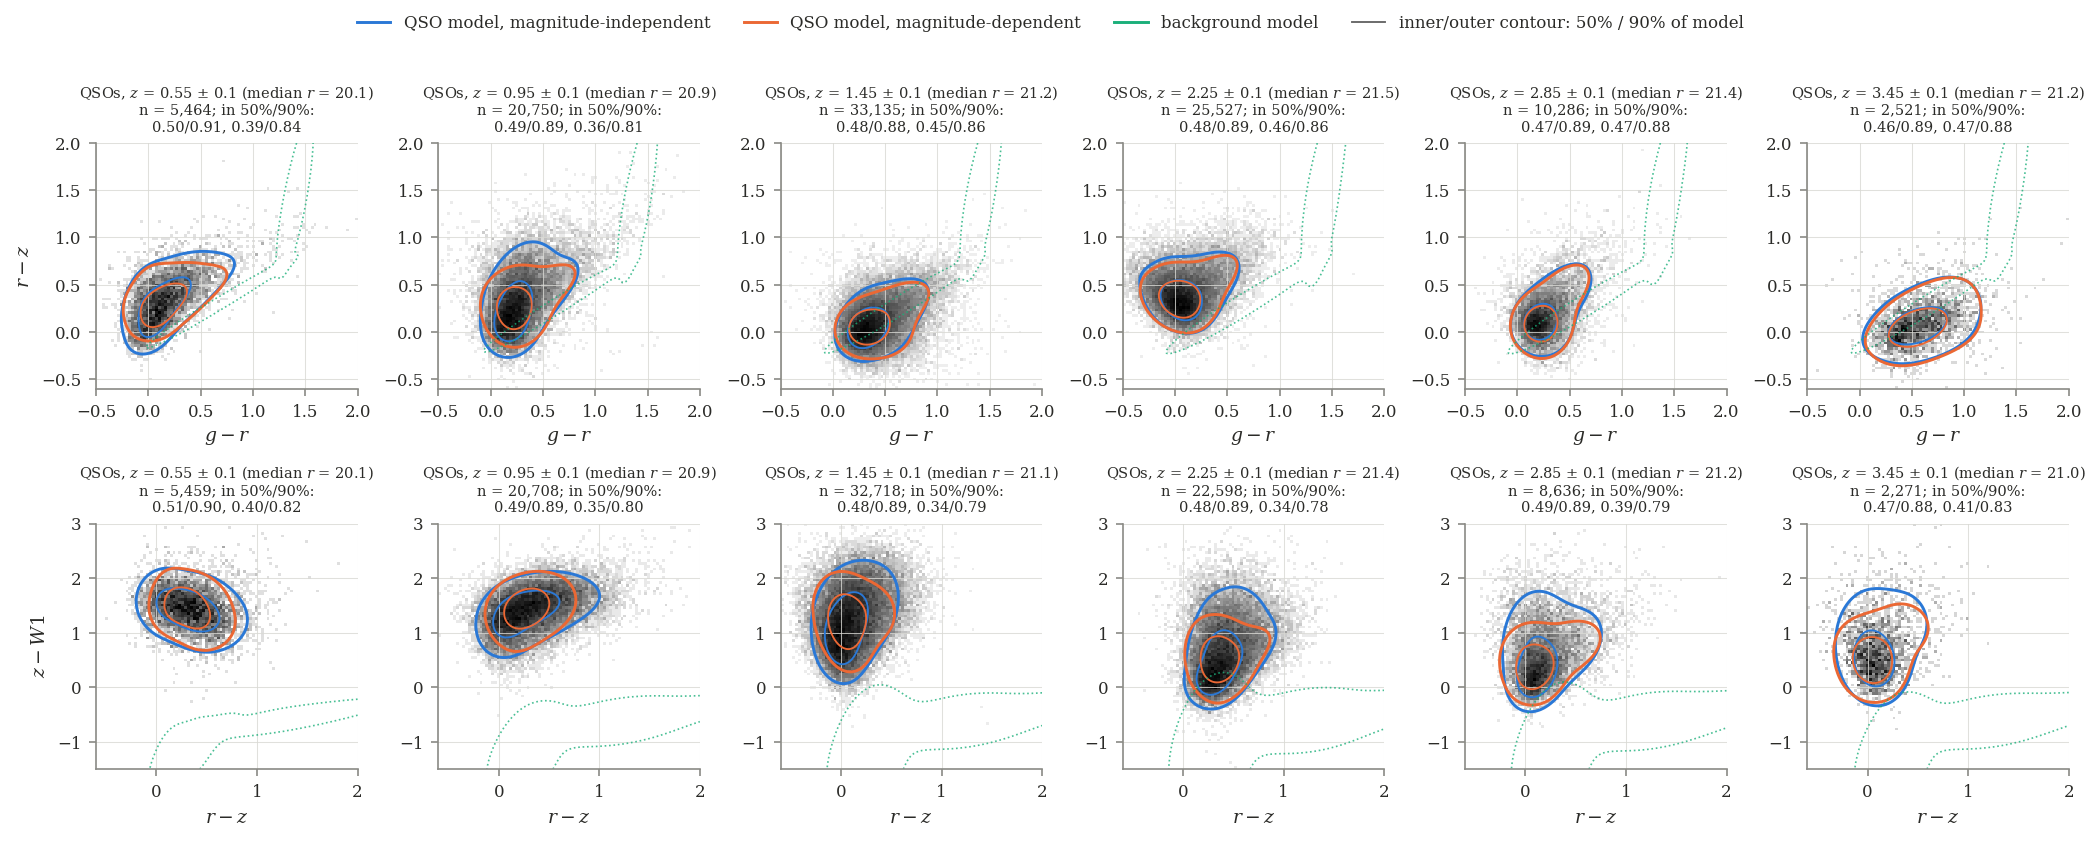
\includegraphics[width=\textwidth]{F09_colour_colour_redshift.png}
\caption{Quasar colour--colour planes in six redshift slices, each conditioned on the slice's median
$r$, with the background model's 90\% contour for reference.}
\label{fig:ccz}
\end{figure}

\subsection{Held-out density}
Per slice, the magnitude-dependent model's kept checkpoint has a held-out density higher than the
magnitude-independent model's by a median 0.666\,nat per object (range 0.381--0.876). Against the
uncorrected 30 September model, the corrected magnitude-dependent model differs by a median
$+0.001$\,nat (range $-0.262$ to $+0.057$). The extinction correction therefore costs essentially
nothing in density, and the density gap between the two quasar models comes from the
magnitude constraint. The quasar models are the same in the promoted and candidate bundles.

\subsection{Ranking against the background: candidate versus promoted bundles}
Table~\ref{tab:compare} compares the candidate bundles with the promoted ones on the same held-out objects
of Section~\ref{sec:perf}, both scored with the faint limit (38,881 quasars; 8,747 background objects
outside the background design tests). The binned background leaves the ranking unchanged and raises
the fraction of quasars given $p_{\rm quasar}>0.5$ in every magnitude bin. On all background objects
the fraction with $p_{\rm quasar}>0.5$ rises slightly, but 400 of these objects are flagged likely quasars;
without them it falls, from 0.32\% to 0.26\% and from 0.29\% to 0.25\%. The support cut keeps the same
fraction of quasars.

\begin{table}[!htbp]\centering\footnotesize
\caption{Promoted (2 October) against candidate bundles on identical held-out rows, faint limit applied.
AUC as defined in Section~\ref{sec:notation}; recall: fraction of test quasars with $p_{\rm quasar}>0.5$;
incidence: fraction of background objects with $p_{\rm quasar}>0.5$, on all background objects and with
the 400 flagged likely quasars removed ($^\ast$; AUC also); kept: support retention.}\label{tab:compare}
\begin{tabular}{llcccccc}
\toprule
QSO model & bundle & AUC & AUC$^\ast$ & recall & incidence & incidence$^\ast$ & kept \\
\midrule
independent & promoted & 0.9752 & 0.9771 & 0.834 & 1.22\% & 0.32\% & 99.53\% \\
            & candidate & 0.9744 & 0.9765 & 0.857 & 1.35\% & 0.26\% & 99.53\% \\
dependent & promoted & 0.9783 & 0.9801 & 0.870 & 1.26\% & 0.29\% & 99.47\% \\
          & candidate & 0.9784 & 0.9804 & 0.889 & 1.44\% & 0.25\% & 99.47\% \\
\bottomrule
\end{tabular}
\end{table}

\subsection{Performance across sky, magnitude, redshift and band coverage}\label{sec:perf}
These tests use 20,000 quasars and 20,000 background objects per hemisphere, drawn before the faint limit
from test-role rows outside every development exclusion and outside the release rows that chose earlier
support thresholds; 38,881 quasars (97.2\%) and 14,247 background objects (35.6\%) pass the faint limit.
Background objects are scored at redshifts drawn from the test quasars' redshifts. The four metrics are
those of Section~\ref{sec:notation}: AUC, held-out density, support retention, and high-QSO incidence,
the fraction of background objects ranked with $p_{\rm quasar}>0.5$. The background test objects include
unidentified quasars, so incidence is not a contamination rate.

\paragraph{Overall.} The AUC is 0.976 (magnitude-independent) and 0.980 (magnitude-dependent); South
0.974 and 0.978, North 0.978 and 0.982. The support cut keeps 99.53\% and 99.47\% of test quasars, in
agreement with the 99.5\% calibration target on rows that did not choose it. High-QSO incidence is 1.07\%
and 1.14\% (South 0.48\% and 0.56\%, North 1.75\% and 1.81\%); the faint limit removes faint stars, which
almost never score high, so these fractions are larger than before the limit.

\paragraph{Sky position and magnitude} (Fig.~\ref{fig:perfsky}). Per-cell AUC is uniform across the
footprint to within a few thousandths. Against $|b|$, AUC is 0.973--0.981 (magnitude-independent) and
0.975--0.985 (magnitude-dependent), highest at the lowest latitudes. Against reference magnitude the two
quasar models differ most for bright quasars: AUC 0.955 against 0.975 at $r<18$ (274 quasars), and 0.979
against 0.990 at $18\le r<19$, where the magnitude-independent model's single colour width is too broad
(Section~\ref{sec:cc}). They converge at $r>21$ (0.969--0.973 against 0.970--0.978).

\paragraph{Redshift} (Fig.~\ref{fig:perfz}). AUC is 0.967--0.980 (magnitude-independent) and 0.976--0.983
(magnitude-dependent) for $0.5\le z_0\le3$, and falls to 0.948 and 0.956 at $z_0=3.45$, where quasar colours
cross the stellar locus. Held-out density falls with redshift as quasars become fainter, and the
magnitude-dependent model stays higher at every redshift. Support retention is above 99\% everywhere.

\paragraph{Band coverage} (Fig.~\ref{fig:perfcov}). Grouping objects by the surveys that observed them mixes
coverage with brightness and redshift, and several groups have fewer than 150 background objects. The
artificial masks score the same objects with fewer bands: Legacy $g,r,z$ only gives AUC 0.979 and 0.980,
all Legacy bands 0.993 and 0.994, all optical bands 0.990 for both. SDSS-only and PS1-only photometry
has no Legacy $r$ and is not scored. The weakest coverage group, SDSS+Legacy South+AllWISE+PS1+NSC
(AUC 0.909 and 0.917, 347 quasars), lies in the NSC region of the southern sky.

\begin{figure}[!htbp]\centering
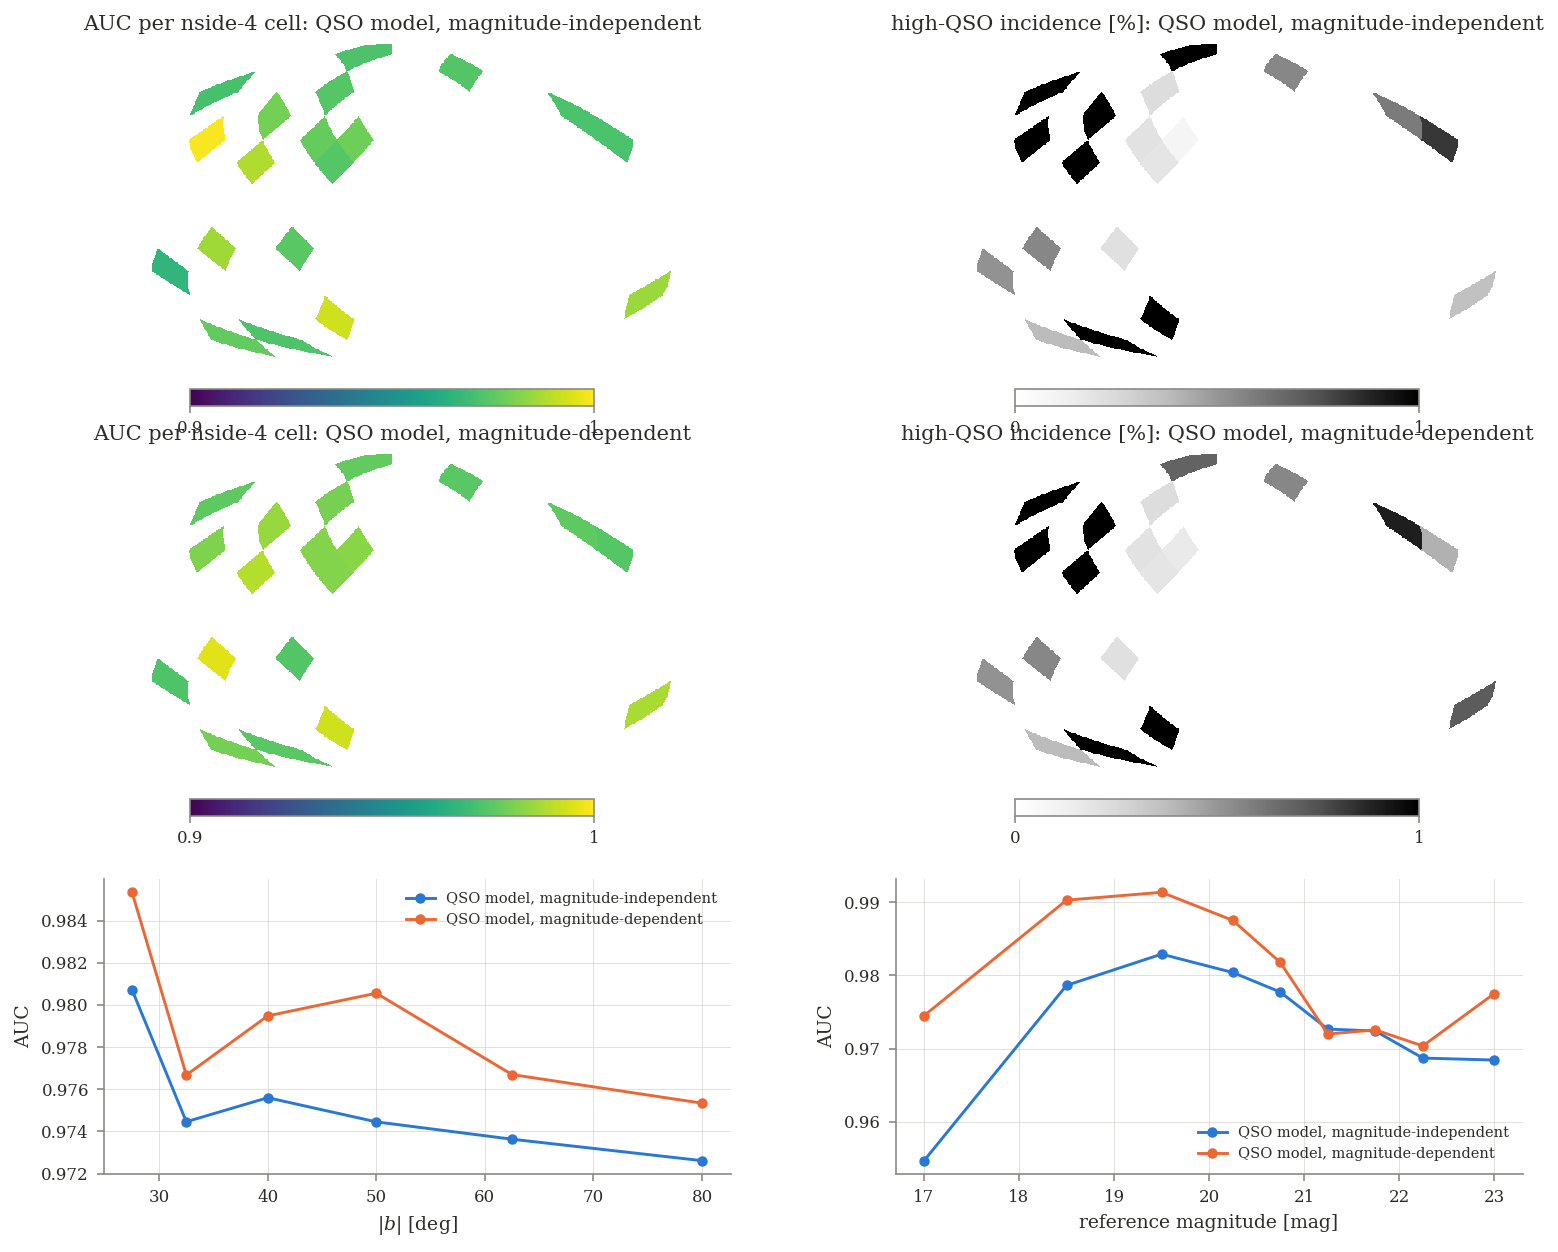
\includegraphics[width=\textwidth]{F12_performance_sky_magnitude.png}
\caption{Performance against sky position and magnitude. Top: AUC and high-QSO incidence per HEALPix
nside-4 cell (cells with at least 30 objects of each class). Bottom: AUC against $|b|$ and against
reference-band magnitude.}
\label{fig:perfsky}
\end{figure}

\begin{figure}[!htbp]\centering
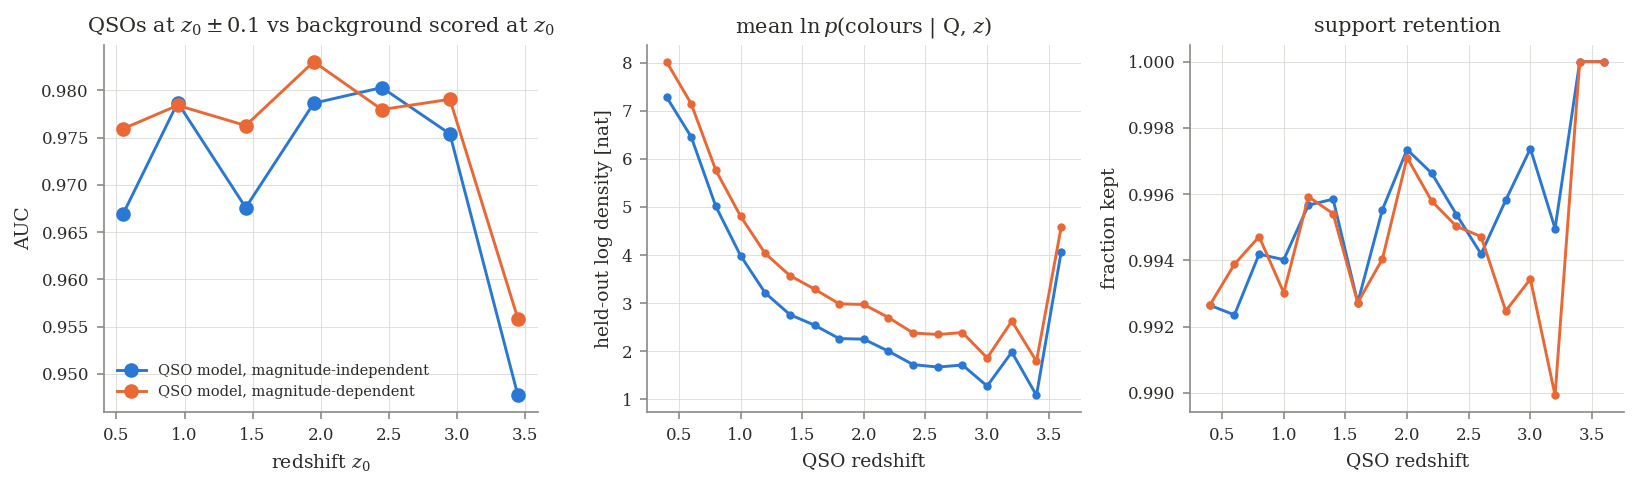
\includegraphics[width=\textwidth]{F13_performance_redshift.png}
\caption{Performance against redshift. Left: AUC of quasars at $z_0\pm0.1$ against background objects
scored at $z_0$. Middle: mean held-out log density of quasars, in bins of their redshift. Right:
support retention.}
\label{fig:perfz}
\end{figure}

\begin{figure}[!htbp]\centering
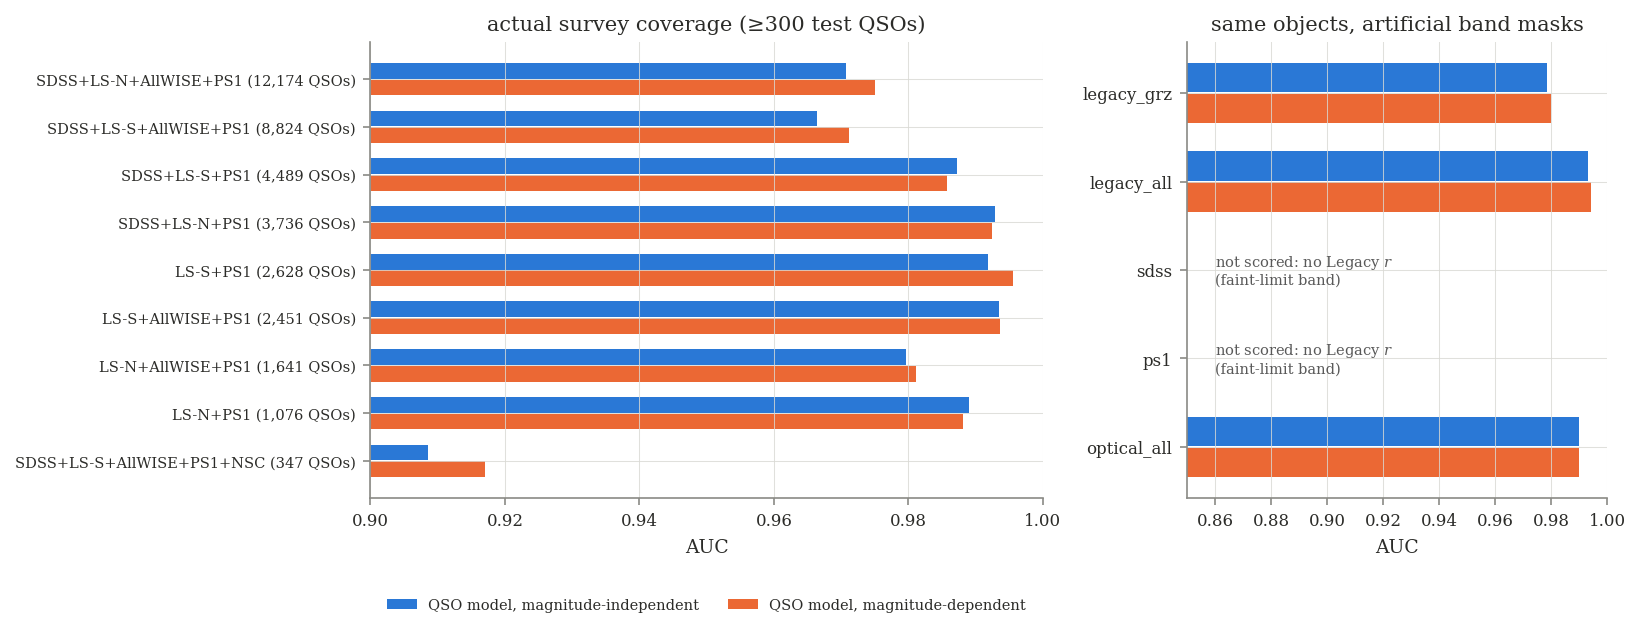
\includegraphics[width=\textwidth]{F14_performance_coverage.png}
\caption{AUC by band coverage. Left: objects grouped by the surveys that observed them (groups with at
least 300 test quasars). Right: the same objects scored with artificial band masks; SDSS-only and PS1-only
objects have no Legacy $r$ and are not scored.}
\label{fig:perfcov}
\end{figure}

\subsection{Artificial colour grids}\label{sec:grids}
A colour grid places synthetic sources on a $15\times15$ lattice in $(g-r,r-z)$ from $-6$ to $8$\,mag at
fixed $r$. These are stress tests of extrapolation into empty colour space, not contamination rates.
In the original low-density region, an unpromoted 30 September candidate gave 72 and 79 high-quasar
points ($p_{\rm quasar}>0.5$) in the North, and the previous model gave 12 at $r=21$. With the
support cut at $2/256$, the magnitude-dependent candidate gives none and the magnitude-independent one
gives one, at South $r=18.5$ (Fig.~\ref{fig:grids}). They abstain from most of the grid: points outside both
models, or rejected by the support cut, are not ranked. Without the support cut the
magnitude-independent model would give 12 high-quasar grid points and the magnitude-dependent one 3
(Fig.~\ref{fig:supportcut}).

\begin{figure}[!htbp]\centering
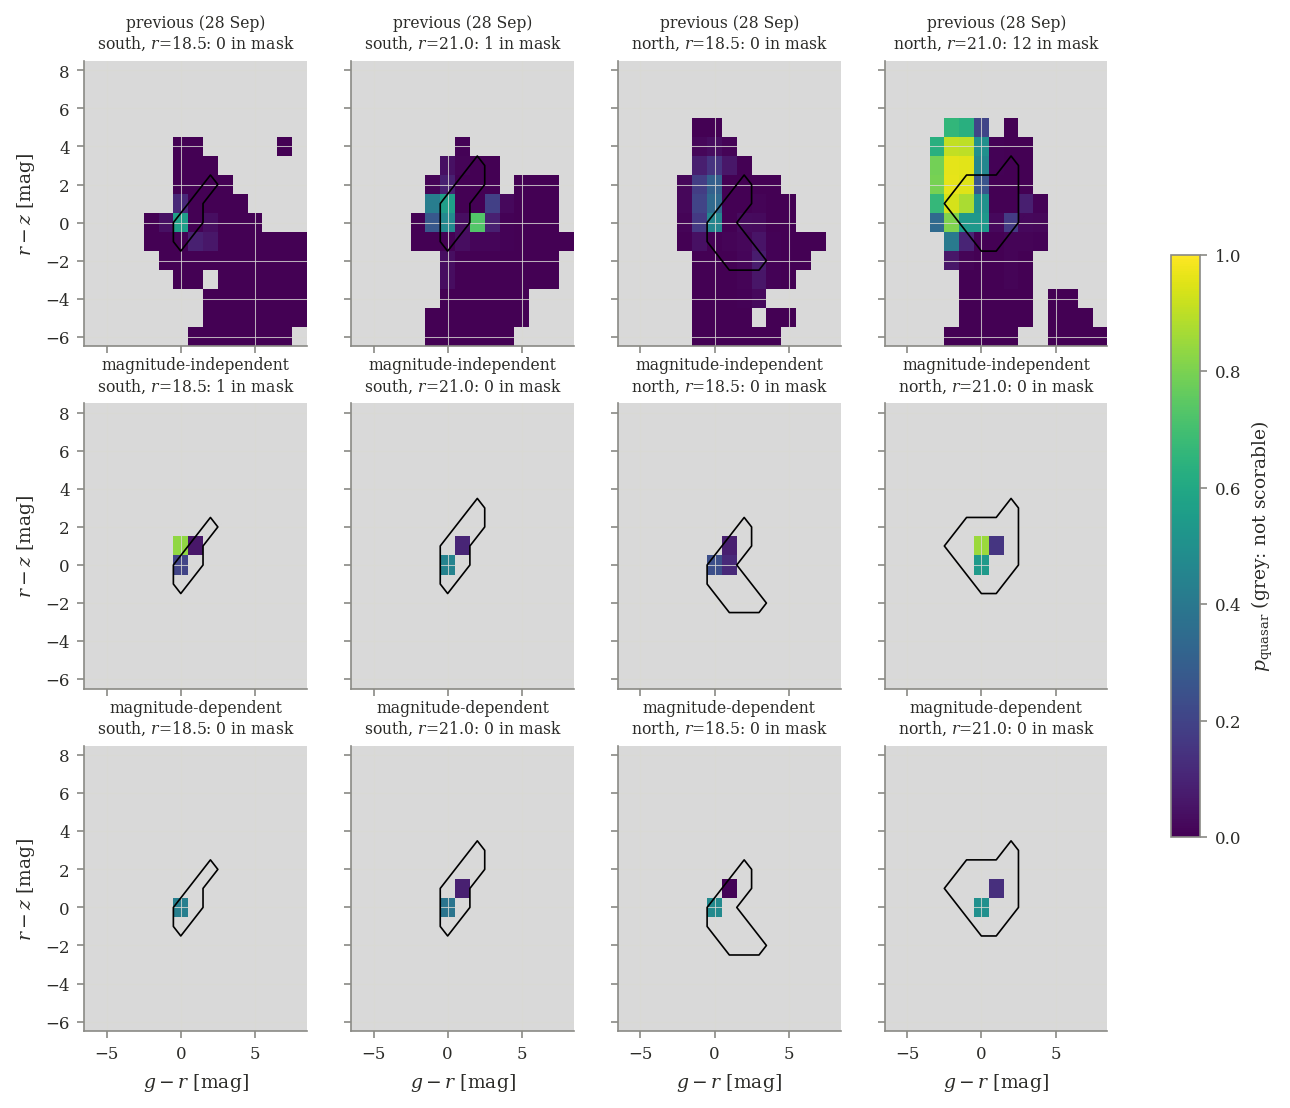
\includegraphics[width=\textwidth]{F15_colour_grids.png}
\caption{Total quasar probability on artificial Legacy colour grids, South and North, $r=18.5$ and 21.
Grey cells are not ranked. Black outline: the original low-density mask.}
\label{fig:grids}
\end{figure}

\subsection{Worked examples}
Figure~\ref{fig:examples} shows six test objects scored by both candidate bundles. For each band the
panels compare the observed corrected luptitude, minus Legacy $r$, with the model's conditional prediction
at the object's redshift. A bright $z=1.51$ quasar, a $z=3.00$ quasar and a $z=0.58$ quasar match their
predictions and receive $p_{\rm quasar}=1.00$ ($\log\R=1.4$--1.6, 0.5--0.6 and 1.5--1.6). One test quasar at
$z=2.26$ has a Legacy $r$ 2--3\,mag fainter than all its other optical bands, a faulty or variable reference
measurement; relative to it the colours are impossible for a quasar, and both models decline to rank it
(support percentile 0.00). A background star has $\log\R=-41.6$ (magnitude-independent);
the magnitude-dependent model rejects it at the support cut. The last panel is a background object that
both models call a quasar ($p_{\rm quasar}=0.99$) but not one at $z_0$ ($\log\R\approx-6$): its colours lie on the
quasar locus at another redshift, and it is probably an unidentified quasar. Legacy and AllWISE $W1,W2$
appear as separate points because Legacy fluxes are AB and AllWISE Vega; the zero points differ by
about 2.7 and 3.3\,mag.

\subsection{Probability calibration}\label{sec:calib}
We test whether $p_{\rm quasar}$ is a calibrated probability on a natural population: all 1,640 known
spectroscopic quasars inside the 49 test cones that pass the faint limit, and 40,000 of the cones'
background objects, weighted by 2.75 to restore their natural share (1.47\% quasars). Objects the scorer
does not rank enter with $p_{\rm quasar}=0$. The background sample still holds unidentified quasars, so the
observed quasar fraction is bracketed by two labellings: known quasars only (a lower bound), and known
quasars plus flagged likely quasars (an upper bound). For both candidate bundles, raw $p_{\rm quasar}$ lies
between the bounds in the mid range ($0.1\lesssim p\lesssim0.95$; Fig.~\ref{fig:calib}). It is too low near
zero (objects at $p<0.01$ contain 0.1--2.5\% quasars) and too high at the top ($p>0.99$: 0.69--0.98
observed). A two-parameter map of the log-odds, fitted on half the cones, is driven by the large $p\approx0$
population and pushes mid-range values below both bounds ($p=0.5\to0.29$), so it is not applied.
$p_{\rm quasar}$ should be read as an approximately calibrated probability whose largest values are
mildly overconfident.

\begin{figure}[!htbp]\centering
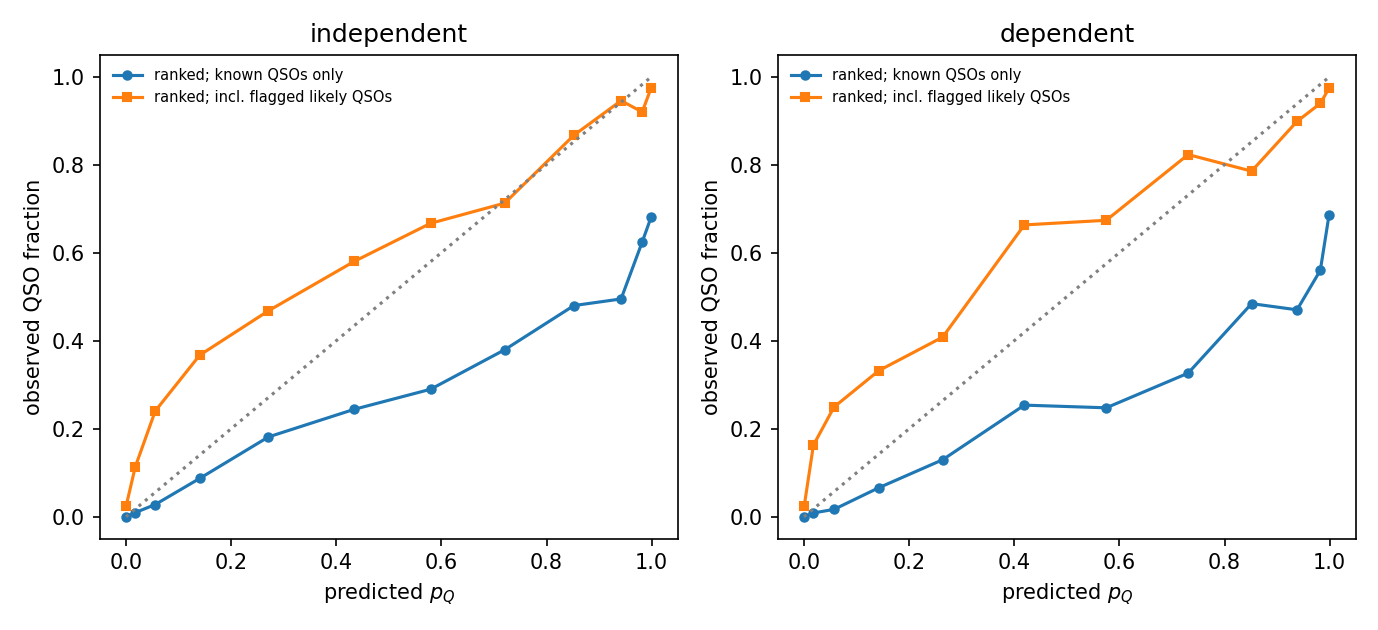
\includegraphics[width=\textwidth]{F18_probability_calibration.png}
\caption{Reliability of $p_{\rm quasar}$ in the 49 test cones (natural population, weighted), for the promoted
(``current'') and candidate (``new'') bundles: observed quasar fraction against mean predicted
$p_{\rm quasar}$ in bins, counting known quasars only (blue, lower bound) or also flagged likely quasars
(orange, upper bound). Dotted: perfect calibration.}
\label{fig:calib}
\end{figure}

\begin{figure}[!htbp]\centering
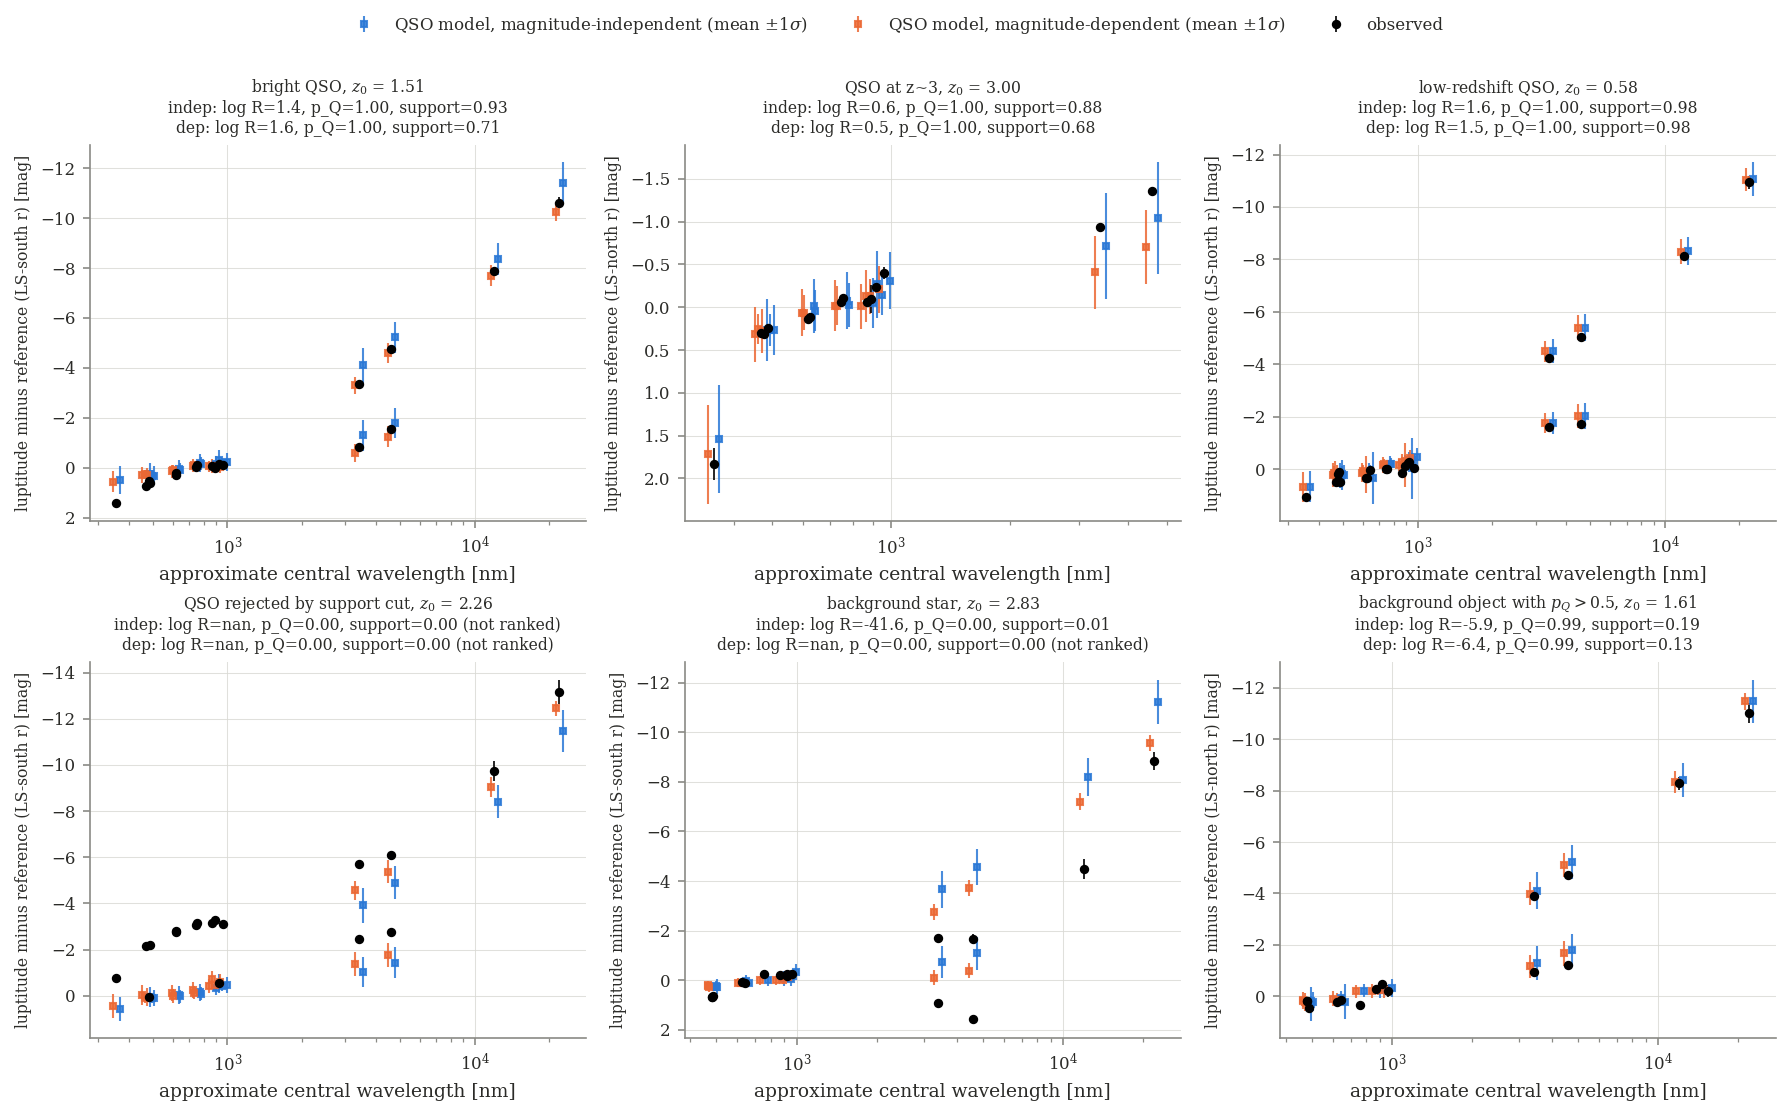
\includegraphics[width=\textwidth]{F16_examples.png}
\caption{Worked examples: observed luptitude minus reference-band luptitude (black) and each model's
conditional prediction at the object's redshift (mean $\pm1\sigma$; blue magnitude-independent, orange
magnitude-dependent). Horizontal positions are approximate central wavelengths, for display only.
Titles give $\log\R$, $p_{\rm quasar}$ and the support percentile from both models. Object identifiers
are in \code{docs/method\_unified/examples.json}.}
\label{fig:examples}
\end{figure}

\clearpage
%======================================================================
\section{Limitations and open items}\label{sec:limits}
%======================================================================
\begin{itemize}
\item \textbf{Probability calibration} is approximate: $p_{\rm quasar}$ is bracketed by the label bounds in
  the mid range and overconfident above 0.97 (Section~\ref{sec:calib}); the reliability of $p_{\rm same}$
  for a narrow redshift window is not tested.
\item \textbf{Background purity.} Faint unidentified quasars not detected by WISE remain in the background
  training sample, and $\Sigma_B$ is counted on the uncleaned sample. The test background sets carry the
  same contamination, which lowers the measured AUC slightly.
\item \textbf{Faint limit.} Sources below Legacy $r$ $S/N=10$, and sources without Legacy $r$, are not scored.
\item \textbf{Selection.} Test quasars share the training selection. Our tests cannot measure the
  intended benefit of the magnitude-independent model for quasars outside DESI and SDSS selection.
\item \textbf{Quasar abundance} is inherited and shifted, not recounted.
\item \textbf{Sparse surveys.} NSC $VR$ and VISTA $Y$ extinction coefficients are approximate, and
  SkyMapper $u,v$ and VHS have little training support.
\item \textbf{Background in the faintest bins} ($r>21.5$) is broader than the data in $W1-W2$ and slightly
  narrower in $r-z$ against $z-W1$ (Fig.~\ref{fig:stellarcc}); these panels hold few WISE-detected stars.
\item \textbf{Promotion.} The candidate bundles are not promoted; the release-check panels of earlier
  notes were not rerun for them (Table~\ref{tab:compare} replaces them).
\item \textbf{Out of scope.} Blends below the separation floor, and a physical-pair clustering prior,
  are deferred.
\end{itemize}

\appendix
%======================================================================
\section{The window factorisation}\label{app:window}
%======================================================================
Write $\Lambda_Q=\int\lambda_Q(z)\,dz$ for the total quasar intensity, and let the declared window $W$
around $z_0$ have effective width $\Delta z_{\rm eff}=\int_Wk(z)\,dz$ for its kernel $k$. The posterior
that the companion is a quasar in the window is
\begin{equation}
p_{\rm same}=\frac{\int_Wk(z)\lambda_Q(z)\,dz}{\Lambda_Q+\lambda_B+\lambda_U}
=\Delta z_{\rm eff}\,\frac{\langle\lambda_Q\rangle_W}{\Lambda_Q+\lambda_B+\lambda_U}\equiv\Delta z_{\rm eff}\,\R,
\end{equation}
with $\langle\lambda_Q\rangle_W$ the kernel-weighted mean over the window. The denominator contains no
window, because $\Lambda_Q$ includes both same-redshift and other-redshift quasars. The scorer integrates
the window on dense nodes at the support boundaries rather than on the coarse redshift grid. For a
window much narrower than the photometric redshift width, $\langle\lambda_Q\rangle_W=\lambda_Q(z_0)$,
which is Eq.~(\ref{eq:R}).

\section{The constrained M step}\label{app:mstep}
For a component with mean $(\mu_m,\vect{\mu}_c)$ and covariance ${\rm diag}(\sigma_m^2,V_c)$, where
$\mu_m$ and $\sigma_m^2$ are fixed, the expected complete-data log likelihood separates into a
magnitude term, constant in the free parameters, and a colour term. Maximising the colour term with
the MAP prior on $V_c$ gives the usual updates applied to the colour block alone. The prior on the full
covariance differs from the prior on $V_c$ by a constant. The constrained update is therefore exact.

\begin{thebibliography}{12}\small
\bibitem[Bovy et al.(2011a)]{Bovy2011XD} Bovy J., Hogg D.~W., Roweis S.~T., 2011, Ann. Appl. Stat., 5, 1657,
  ``Extreme deconvolution'', \href{https://arxiv.org/abs/0905.2979}{arXiv:0905.2979}.
\bibitem[Bovy et al.(2011b)]{Bovy2011XDQSO} Bovy J. et al., 2011, ApJ, 729, 141, ``Think outside the color box'' (XDQSO),
  \href{https://arxiv.org/abs/1011.6392}{arXiv:1011.6392}.
\bibitem[Kang et al.(2025)]{Kang2025} Kang Y., Hennawi J.~F., Schindler J.-T., Tamanas J., Nanni R., 2025,
  MNRAS, 541, 2815, ``Extreme deconvolution reimagined'' (CondXD),
  \href{https://doi.org/10.1093/mnras/staf1068}{doi:10.1093/mnras/staf1068}.
\bibitem[Lupton et al.(1999)]{Lupton1999} Lupton R.~H., Gunn J.~E., Szalay A.~S., 1999, AJ, 118, 1406,
  \href{https://arxiv.org/abs/astro-ph/9903081}{arXiv:astro-ph/9903081}.
\bibitem[Lyke et al.(2020)]{Lyke2020} Lyke B.~W. et al., 2020, ApJS, 250, 8, SDSS DR16Q,
  \href{https://arxiv.org/abs/2007.09001}{arXiv:2007.09001}.
\bibitem[Schlegel et al.(1998)]{SFD98} Schlegel D.~J., Finkbeiner D.~P., Davis M., 1998, ApJ, 500, 525,
  \href{https://doi.org/10.1086/305772}{doi:10.1086/305772}.
\bibitem[Schlafly \& Finkbeiner(2011)]{SF11} Schlafly E.~F., Finkbeiner D.~P., 2011, ApJ, 737, 103,
  \href{https://doi.org/10.1088/0004-637X/737/2/103}{doi:10.1088/0004-637X/737/2/103}.
\bibitem[Stern et al.(2012)]{Stern2012} Stern D. et al., 2012, ApJ, 753, 30, ``Mid-infrared selection of AGN with WISE'',
  \href{https://doi.org/10.1088/0004-637X/753/1/30}{doi:10.1088/0004-637X/753/1/30}.
\bibitem[Storey-Fisher et al.(2024)]{StoreyFisher2024} Storey-Fisher K. et al., 2024, ApJ, 964, 69, Quaia,
  \href{https://doi.org/10.3847/1538-4357/ad1328}{doi:10.3847/1538-4357/ad1328}.
\bibitem[Wolf et al.(2018)]{Wolf2018} Wolf C. et al., 2018, PASA, 35, e010, SkyMapper DR1,
  \href{https://doi.org/10.1017/pasa.2018.5}{doi:10.1017/pasa.2018.5}.
\bibitem[Legacy Surveys(2020)]{LSDR9} Legacy Surveys DR9 catalogue documentation, Galactic extinction coefficients,
  \url{https://www.legacysurvey.org/dr9/catalogs/}.
\end{thebibliography}
\end{document}
